\clearpage 
\section{Charge flip details}
\label{app:flips}
\subsection{Comparison of charge flip rates in different MC productions}

\par{\bf Monte Carlo comparison study}

To validate our choice of control region, we apply the likelihood fit method to a pure $Z \to e^+e^-$ MC sample in order to compare the results with the ones obtain by running on data. This study compares the charge flip rates extracted from different MC samples especially MC12 and MC15 ones, at $\sqrt{s}=8$ TeV and $\sqrt{s}=13$ TeV respectively. The goal of such study is to look if the amount of mis-identified electrons increased in Run 2 with respect to Run 1. The reproduction of Run 1 results is also a good way to cross-check our new likelihood fit method.

A total of 4 different samples will be use in this study: MC12, DC14, MC15, MC12r20. The MC12 and MC15 samples are the most important ones and they correspond official Monte Carlo simulated events, respectively for Run 1 and Run 2 analyses. The DC14 sample is similar to MC15 one, but it was mainly used to produce some Run 2 projection results. Finally, the MC12r20 sample (standing for \textit{MC12 release 20}) is a sample using the Run 1 energy ($\sqrt{s}=8$ TeV) and detector geometry (no IBL), but using a Run 2 reconstruction based on the latest recommendations included in release 20. The purpose of such a sample is to disentangle the combined effects due to detector geometry and reconstruction by using the same geometry as the MC12 sample but the same reconstruction as the MC15 sample. The motivations to study a sample like that will be explained below.

%------------------------------------------------
\begin{table}[!htb]
\centering
\begin{tabular}{|l|c|c|}
\hline
 & Electrons & Jets \\
\hline \hline
Acceptance & $\pt$ > 10 GeV & $\pt$ > 20 GeV \\
		   & $\eta$ < 2.47 & $\eta$ < 2.8 (< 2.5 for b-jets) \\ 
\hline
PID 		   & \texttt{mediumPP} \small (MC12) & \_ \\
  		   & \texttt{LooseLLH} \small (DC14, MC15, MC12r20) &  \\
\hline
b-tagging	   & \_ & \small MV1 > 0.98, 70\% (MC12, DC14) \\
           	   &  & \small MV2c20 > -0.5911, 80\% (MC15, MC12r20) \\
\hline
\end{tabular}
\caption{\label{tab:baseline} Electrons, jets and b-jets baseline selection cuts for different MC samples.}
\end{table}
%------------------------------------------------

The baseline selection cuts for different objects (electrons, jets and $b$-jets) are described in Table \ref{tab:baseline}. The fact that PID requirements for electrons as well as $b$-tagging requirements for $b$-jets are not the same between different MC samples is due to the improvement of some variables between the Run 1 and Run 2 configurations. In Table~\ref{tab:baseline} the efficiency associated to the MV1 variable is 70\% and 80\% for MV2c20 variable. 

%------------------------------------------------
\begin{table}[!htb]
\centering
\begin{tabular}{|l|c|c|}
\hline
 & MC12 & DC14, MC15, MC12r20 \\
\hline \hline
PID  & \texttt{TightPP}  & \texttt{TightLLH} \\
\hline
Track isolation & $pTcone20/\pt<0.06$ & $pTvarcone20/\pt<0.06$ \\
\hline
Calorimeter isolation & \multicolumn{2}{|c|}{$topoETcone20/\pt<0.06$} \\
\hline
Impact parameter & \multicolumn{2}{|c|}{$\left | z_0 \cdot \sin{\theta} \right |<0.4 mm $} \\
 &  \multicolumn{2}{|c|}{$\left | d_0 / \sigma(d_0) \right |<3.0$} \\
\hline
\end{tabular}
\caption{\label{tab:signal} Signal selection cuts applied on $Z\to e^+e^-$ events on top of overlap removal procedure for different MC samples.}
\end{table}
%------------------------------------------------

Using the pair formed by the two signal leading electrons, one can now count the number of SS and OS pairs along all $Z\to e^+e^-$ events and used those numbers as inputs in the likelihood method defined above in order to extract the nominal charge flip rates in different MC samples.

The left plot on Fig.~\ref{fig:12vs15} compares the charge flip rates between three MC samples: MC12, DC14 and MC15 for 6 different $\eta$ bins and $30<\pt<40$ GeV, while the right plot shows the ratios between MC15 and MC12 charge flip rates with the same binning. Similar plots corresponding to 8 other $\pt$ bins can be found in Appendix~\ref{app:CFrates1}. For both plots, only statistical errors are shown. For the majority of the 54 total bins the ratio is positive and greater than 2.0 (vary between 0.5 and 8.0), meaning that the charge flip rates from MC15 are often twice as large as charge flip rates from MC12 sample.

%------------------------------------------------
\begin{figure}[!htb]
\begin{center}
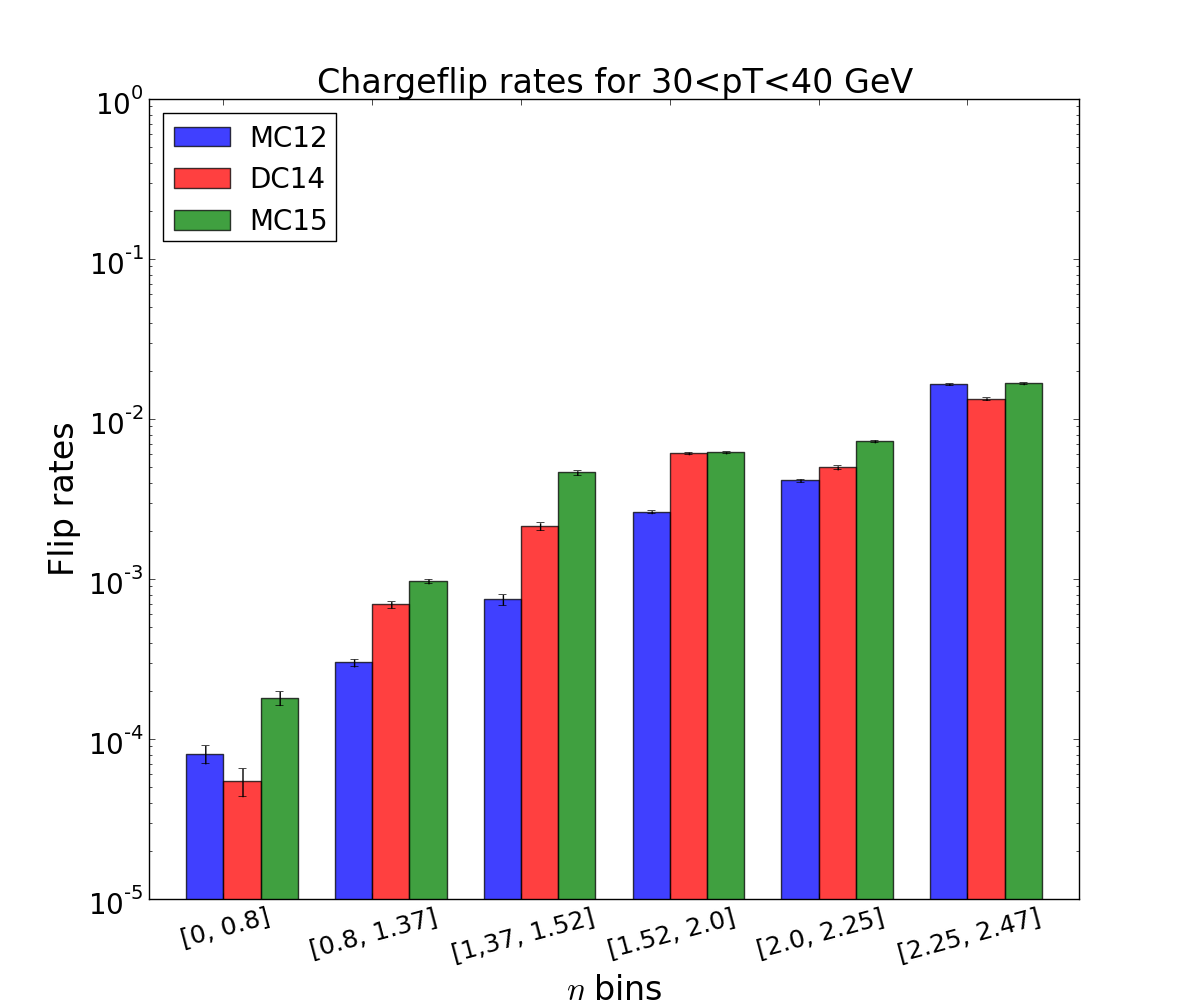
\includegraphics[width=0.4\linewidth]{FIGURES/BKG/chargeFlip/APPENDIX/fliprates_MC12/fliprates_3samples_30.png}
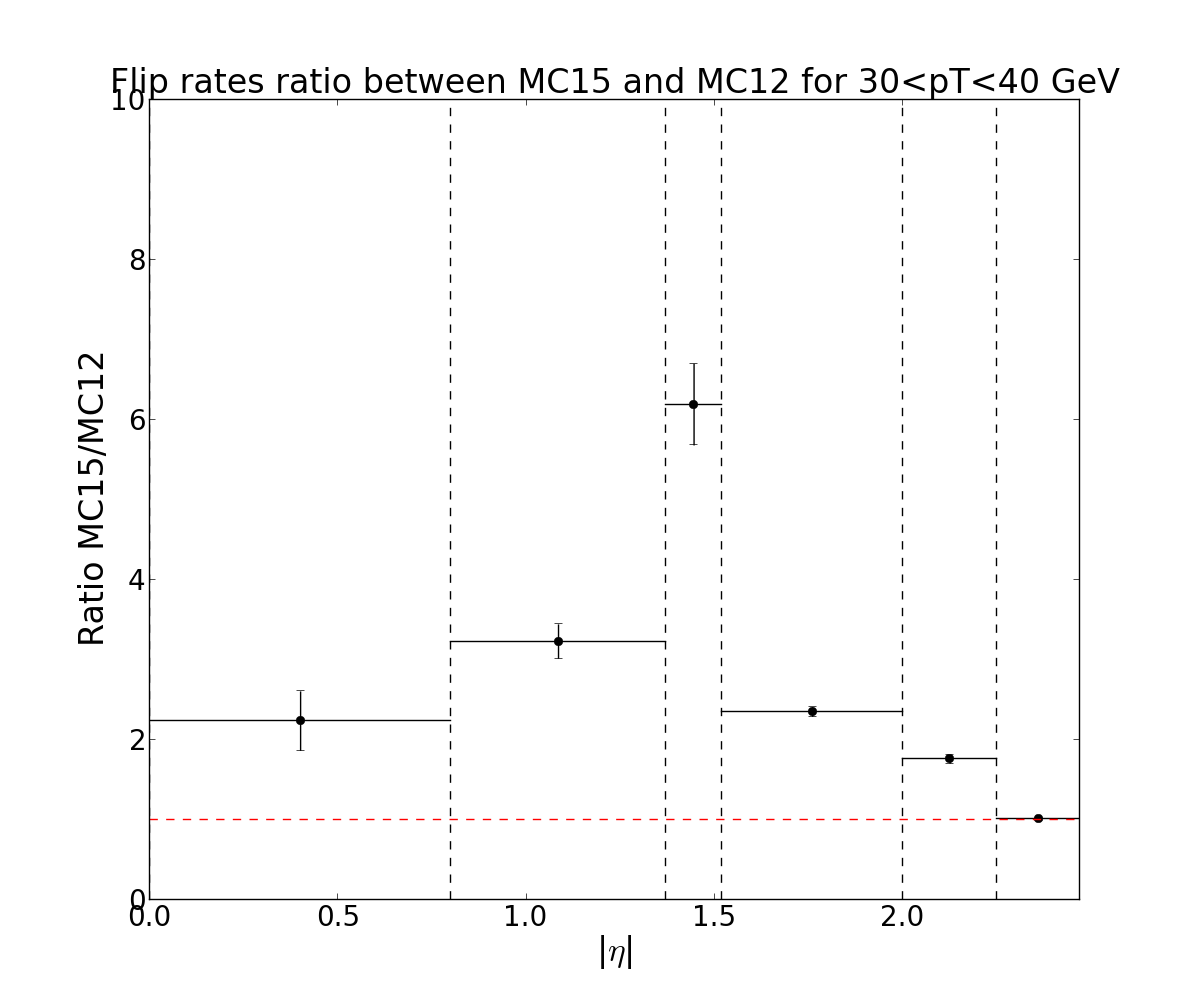
\includegraphics[width=0.4\linewidth]{FIGURES/BKG/chargeFlip/APPENDIX/ratio_MC15vsMC12/ratio_plot_30.png}
\end{center}
\caption{\label{fig:12vs15} Left plot: Charge flip rates extracted from MC12 sample in blue, DC14 sample in red and MC15 in green. The rates are computed for 6 different $\eta$ bins and one $\pt$ bin ($30<\pt<40$ GeV), only statistical uncertainties are shown. Right plot: Ratios between MC15 and MC12 charge flip rates with the same binning of left plot, only statistical uncertainties are shown.}
\end{figure}
%------------------------------------------------

The right plot on Fig.~\ref{fig:12vs15} clearly shows that the charge flip rates extracted from an MC15 sample are generally greater than the ones extracted from an MC12 sample. The two main effects that may have changes from MC12 to MC15 are the reconstruction of the event (object definition, variables, etc.) and the geometry of the ATLAS detector, which is different with the new IBL tracking system installed for Run 2. The amount of material added in Run 2 (IBL and services), but also the position of the IBL, may have increased the charge mis-measurement rate because if the track curvature change direction early (near to the collision point) the odds of mis-identified the charge are greater than in the case where the track curvature is modified later during its path. To be able to distinguish between those two possible effects, a new MC sample was used (MC12r20), a sample based on Run 1 geometry (no IBL) but with Run 2 reconstruction. By comparing this sample to the MC12 and/or MC15 ones, it was easier to distinguish whether geometry or reconstruction was the most influential on the charge flip rate measurement.

%------------------------------------------------
\begin{figure}[!htb]
\begin{center}
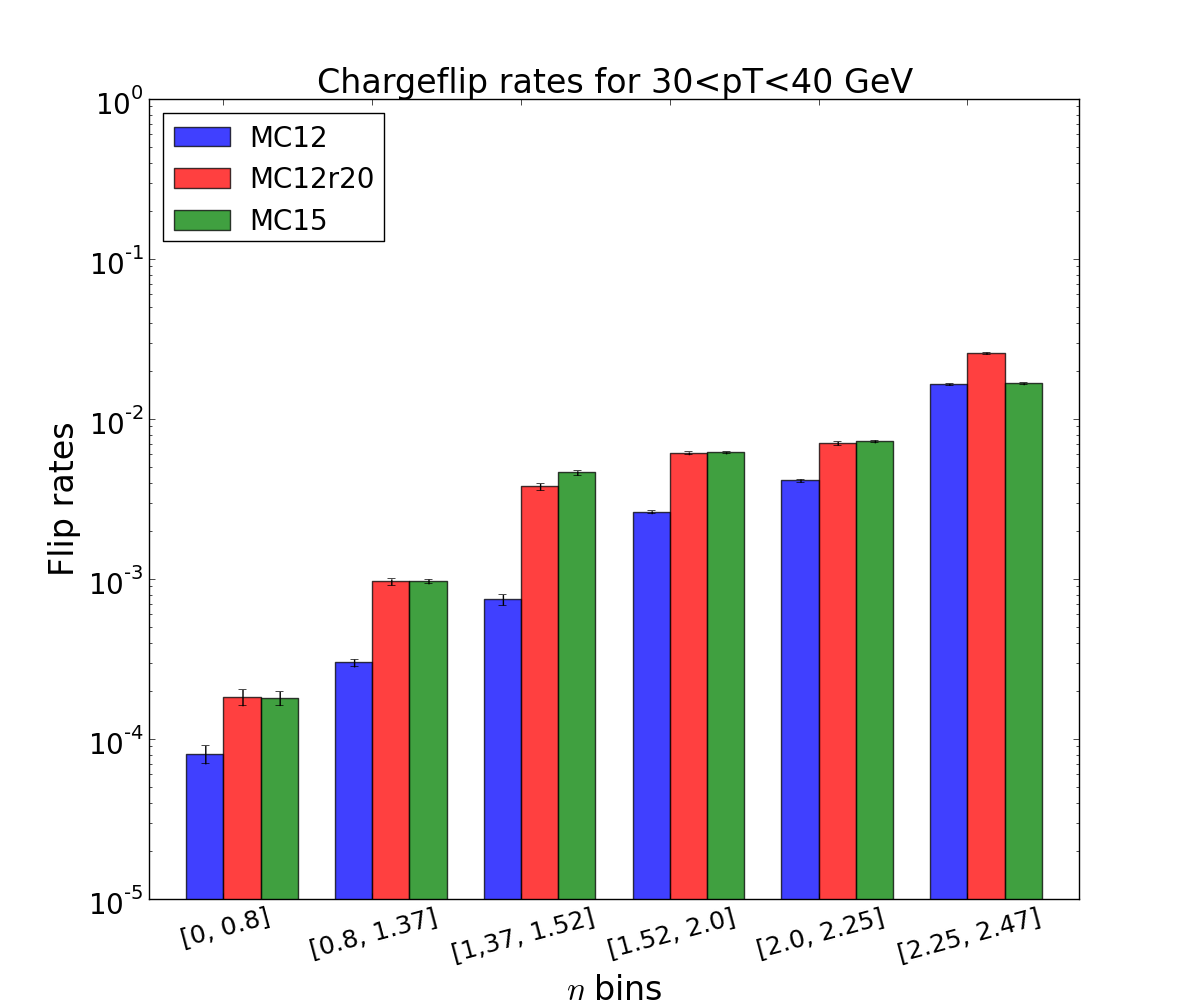
\includegraphics[width=0.4\linewidth]{FIGURES/BKG/chargeFlip/APPENDIX/fliprates_MC12r20/fliprates_3samples_30.png}
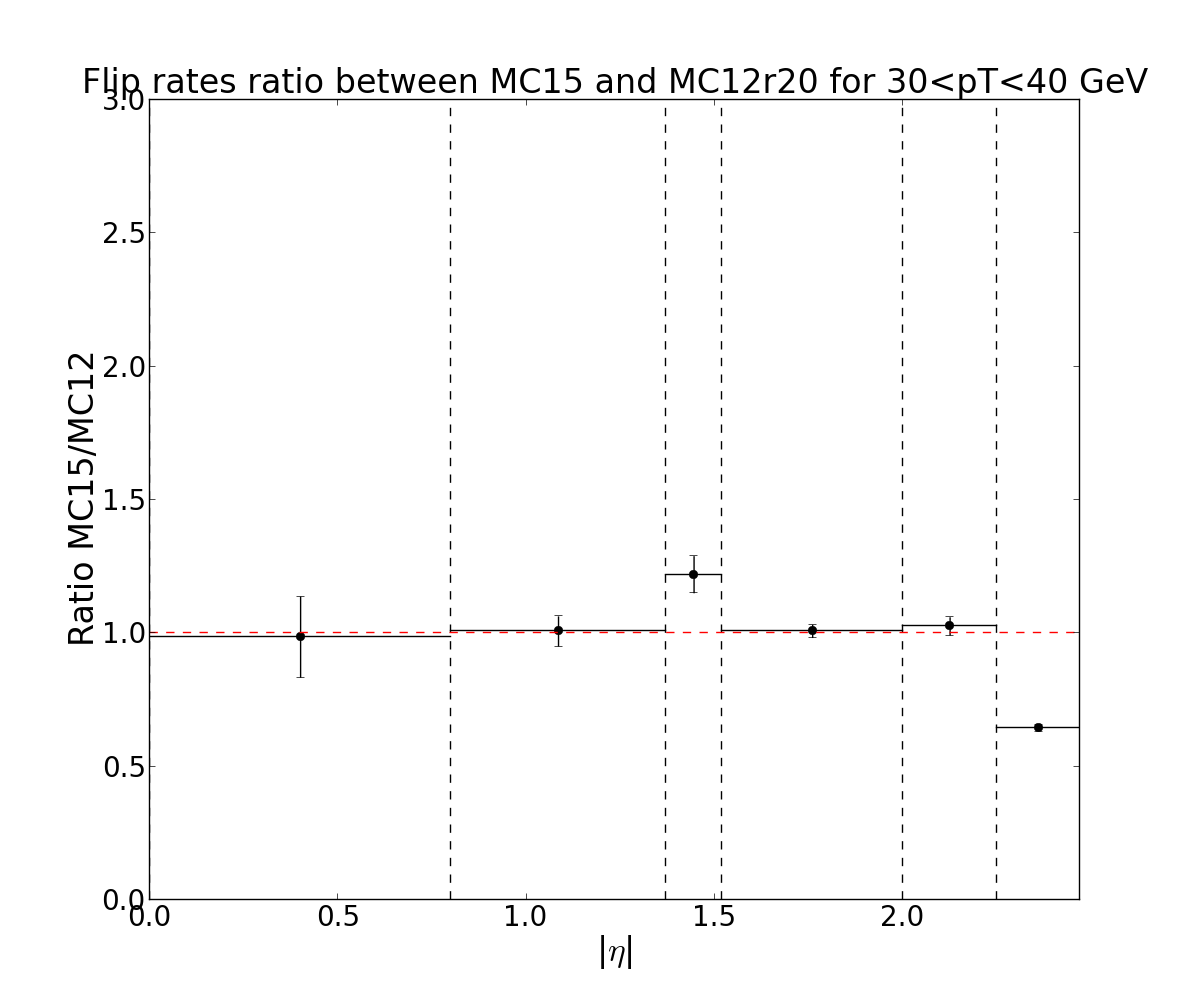
\includegraphics[width=0.4\linewidth]{FIGURES/BKG/chargeFlip/APPENDIX/ratio_MC15vsMC12r20/ratio_plot_30.png}
\end{center}
\caption{\label{fig:12r20vs15} Left plot: Charge flip rates extracted from MC12 sample in blue, MC12r20 sample in red and MC15 in green. The rates are computed for 6 different $\eta$ bins and one $\pt$ bin ($30<\pt<40$ GeV), only statistical uncertainties are shown. Right plot: Ratios between MC15 and MC12r20 charge flip rates with the same binning of left plot, only statistical uncertainties are shown.}
\end{figure}
%------------------------------------------------

This comparison is shown in Fig.~\ref{fig:12r20vs15}, again for 6 different $\eta$ bins are and one $\pt$ bin ($30<\pt<40$ GeV), comparing the charge flip rates extracted from MC12, MC12r20 and MC15 samples on left plot and the charge flip rates ratio between MC15 and MC12r20 on right plot. Again, similar plots corresponding to 8 other $\pt$ bins can be found in Appendix~\ref{app:CFrates2}. On those plots, one can see that the computed ratio varies between 0.5 and 2.0 over the 54 total possible bins but in most cases the ratio is $\approx 1.0$. By comparing those two samples which use the same reconstruction, we disentangled geometry and reconstruction and with the results shown on the right plot of Fig.~\ref{fig:12r20vs15}, it is possible to conclude that the new geometry is not the main cause creating an increase in the charge flip rates as seen on left plot in Fig.~\ref{fig:12vs15}. Nevertheless, we cannot assume that difference in geometry has no effect at all on the charge mis-measurement rates since the ratios between MC12r20 and MC15 samples are not in perfect agreement with 1.0, but it is clearly less relevant compared to difference in reconstruction.

The origin of a disagreement between MC12 and MC15 samples coming from the reconstruction can be studied by looking at different variables used in the signal selection cuts in Table~\ref{tab:signal}. In order to understand which variables among PID, track and calorimeter isolation, longitudinal and transverse impact parameter are associated to the disagreement, one can compute the charge flip rates by applying only one of the cuts presented in Table~\ref{tab:signal}, rather than applying all the signal selection cuts on both electrons forming the pair. This was done for two specific binning, the first one composed of 9 $\pt$ bins between the range [20, 150] GeV and only one $\eta$ bin ([0, 2.47]), while the second composed of 6 $\eta$ bins between the range [0, 2.47] and only one $\pt$ bin ([20, 150] GeV). 

The top plots of Fig.~\ref{fig:all} show the charge flip rates for those two sets of bins when all signal cuts are applied. One can easily see that the rates computed with MC12 sample are lower in each bin than the one computed with MC15 sample. The middle and bottom plots present the same results but only when the PID or $d_0$ requirements are applied. It is clear that the $d_0$ significance variable strongly affect the charge flip rate measures. This effect leads to an increase in the MC15 results with respect to MC12 ones of a factor $\sim 2$ in the $\pt$ binned bottom left plot. The middle plots show a different behavior while the MC12 charge flip rates are almost always greater than the one from other samples in each $\pt$ or $\eta$ bins. This could be understood as the fact that the PID requirement used in MC15 sample (\texttt{TightLLH}) is tighter than the one used in MC12 sample (\texttt{TightPP}), which reduces the rates. The increasing rates in MC12 sample for $\pt$ bellow 60 GeV in the middle left plot was not an expected feature and it is not clear yet why there is such a pattern at low $\pt$. Other similar plots using whether only track isolation, calorimeter isolation or longitudinal impact parameter as signal selection variables have been done and are presented in Appendix \ref{app:CFrates3}. In those plots, one can still see an increase between MC15 and MC12 charge flip rates, but the difference is rather small compared to the one due to $d_0$ significance cut (bottom left plot on Fig. \ref{fig:all}).

%------------------------------------------------
\begin{figure}[!htbp]
\begin{center}
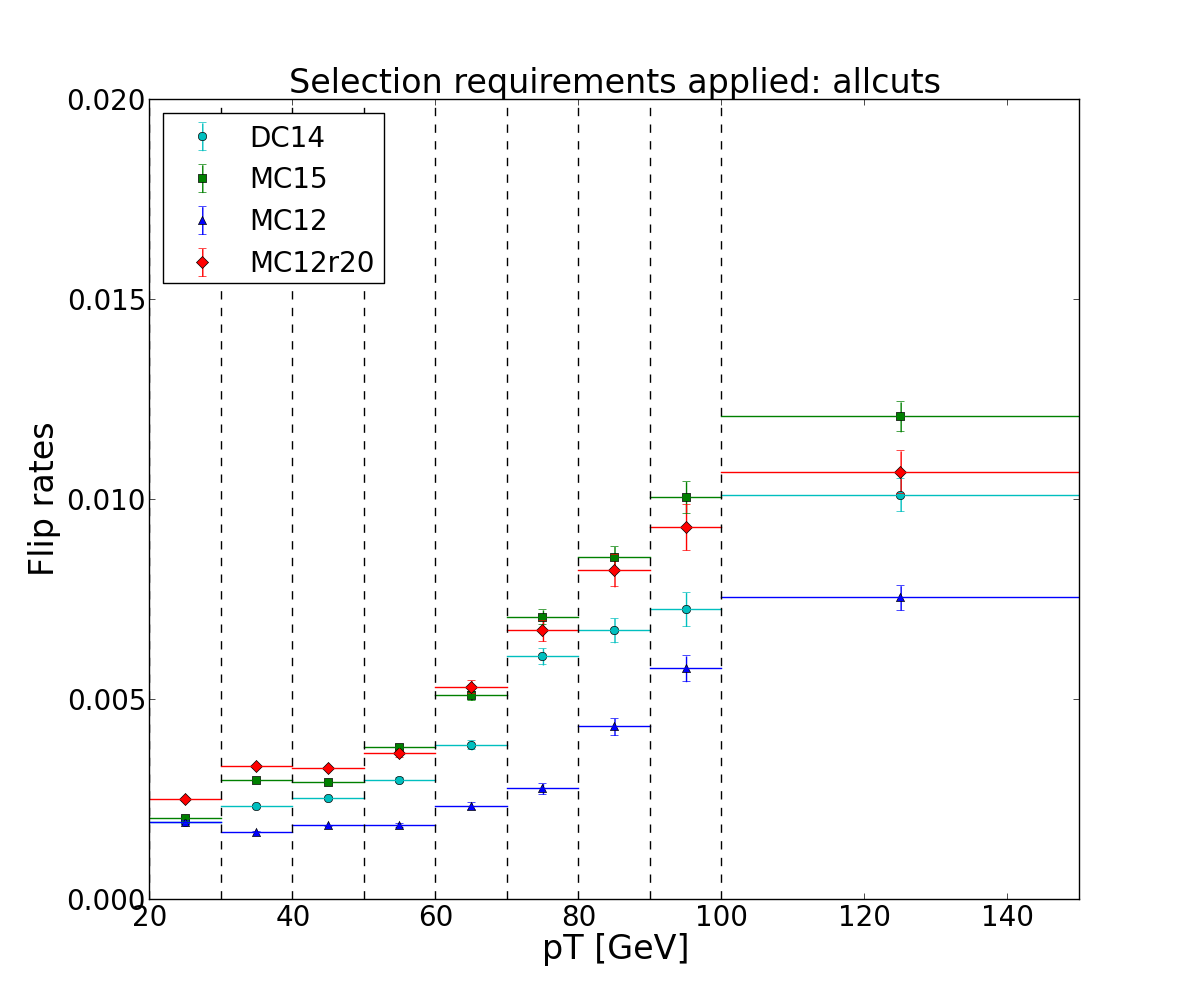
\includegraphics[width=0.4\linewidth]{FIGURES/BKG/chargeFlip/APPENDIX/fliprates_pT_allcuts.png}
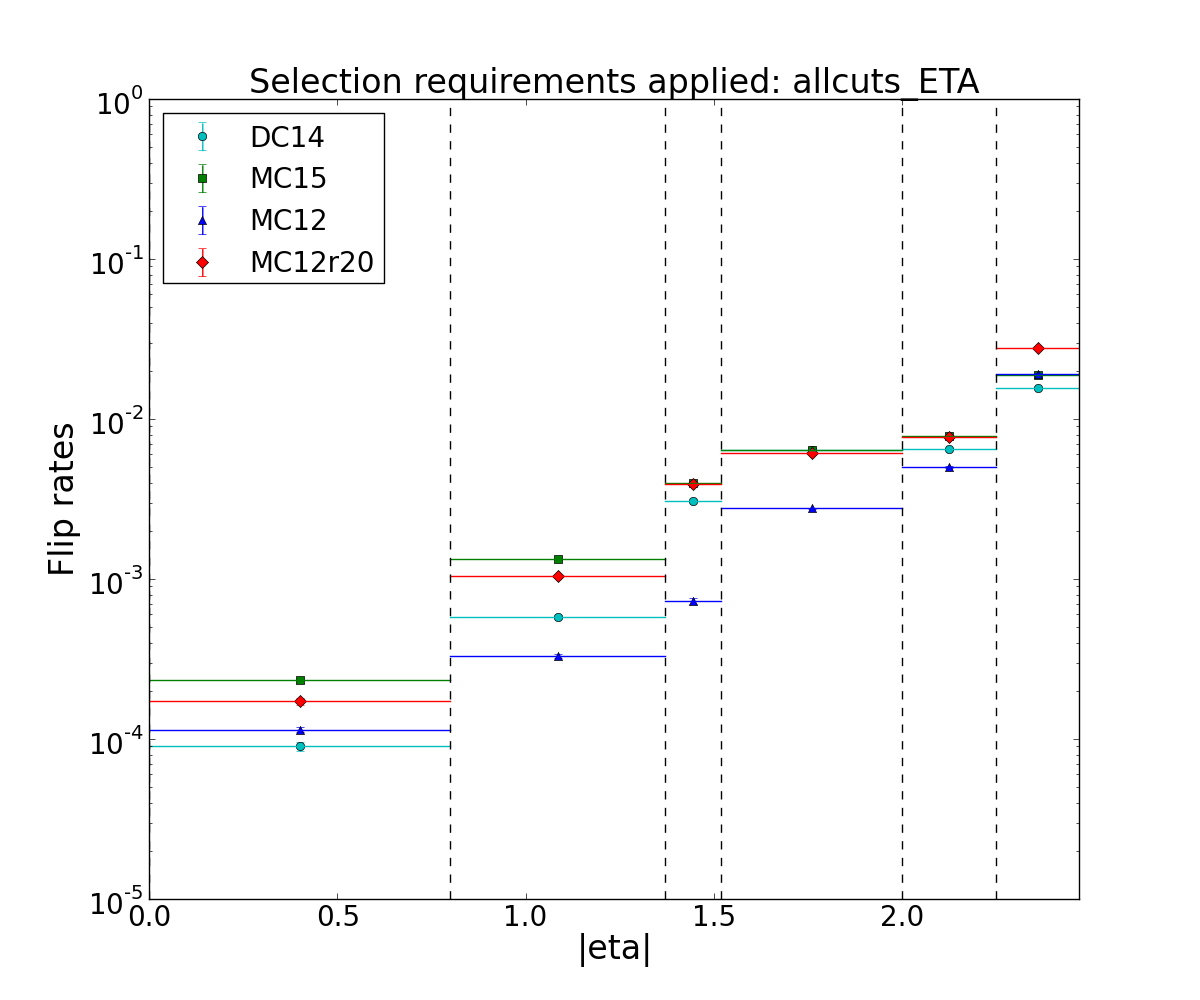
\includegraphics[width=0.4\linewidth]{FIGURES/BKG/chargeFlip/APPENDIX/fliprates_eta_allcuts_ETA.png}
\vfill
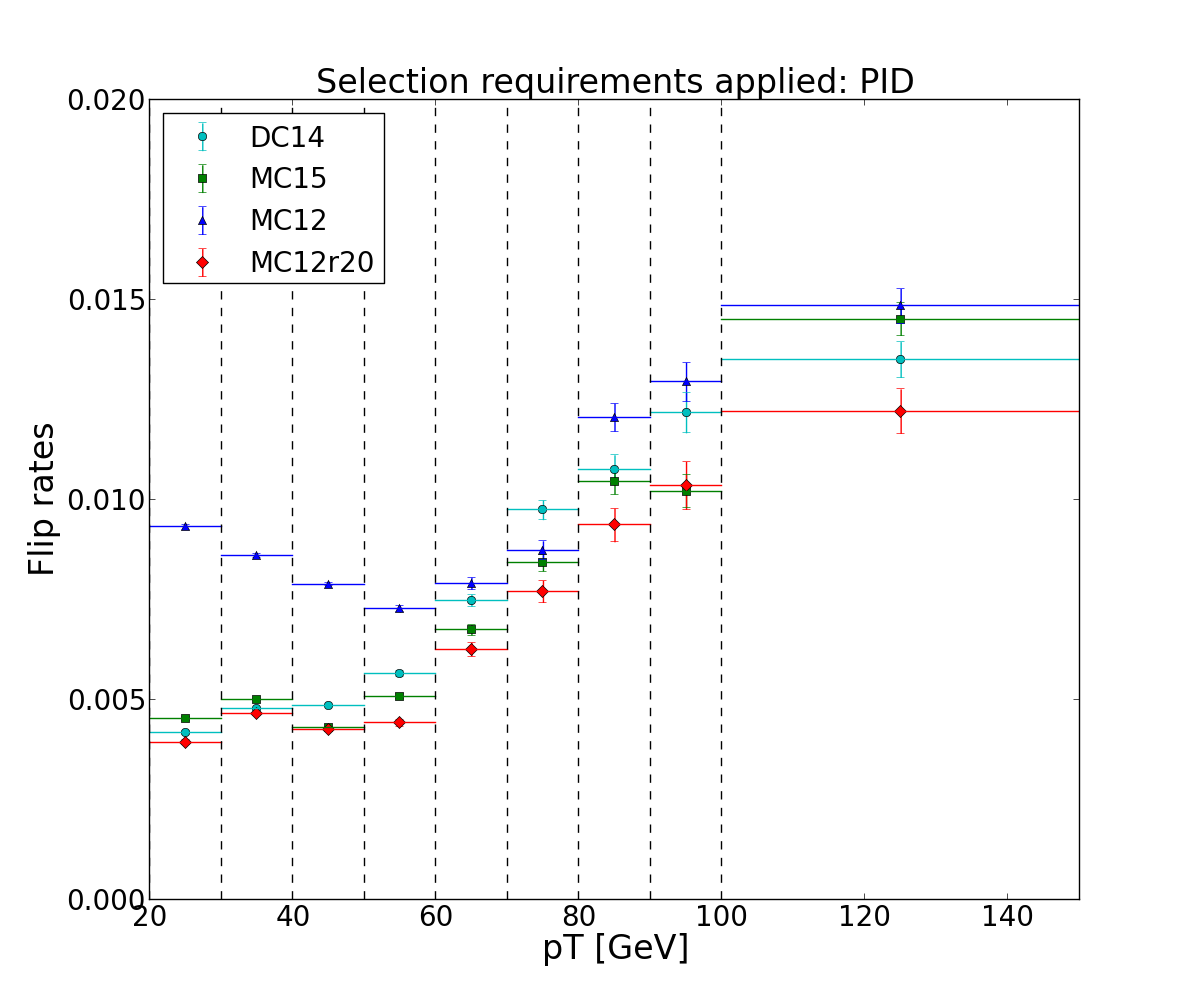
\includegraphics[width=0.4\linewidth]{FIGURES/BKG/chargeFlip/APPENDIX/fliprates_pT_PID.png}
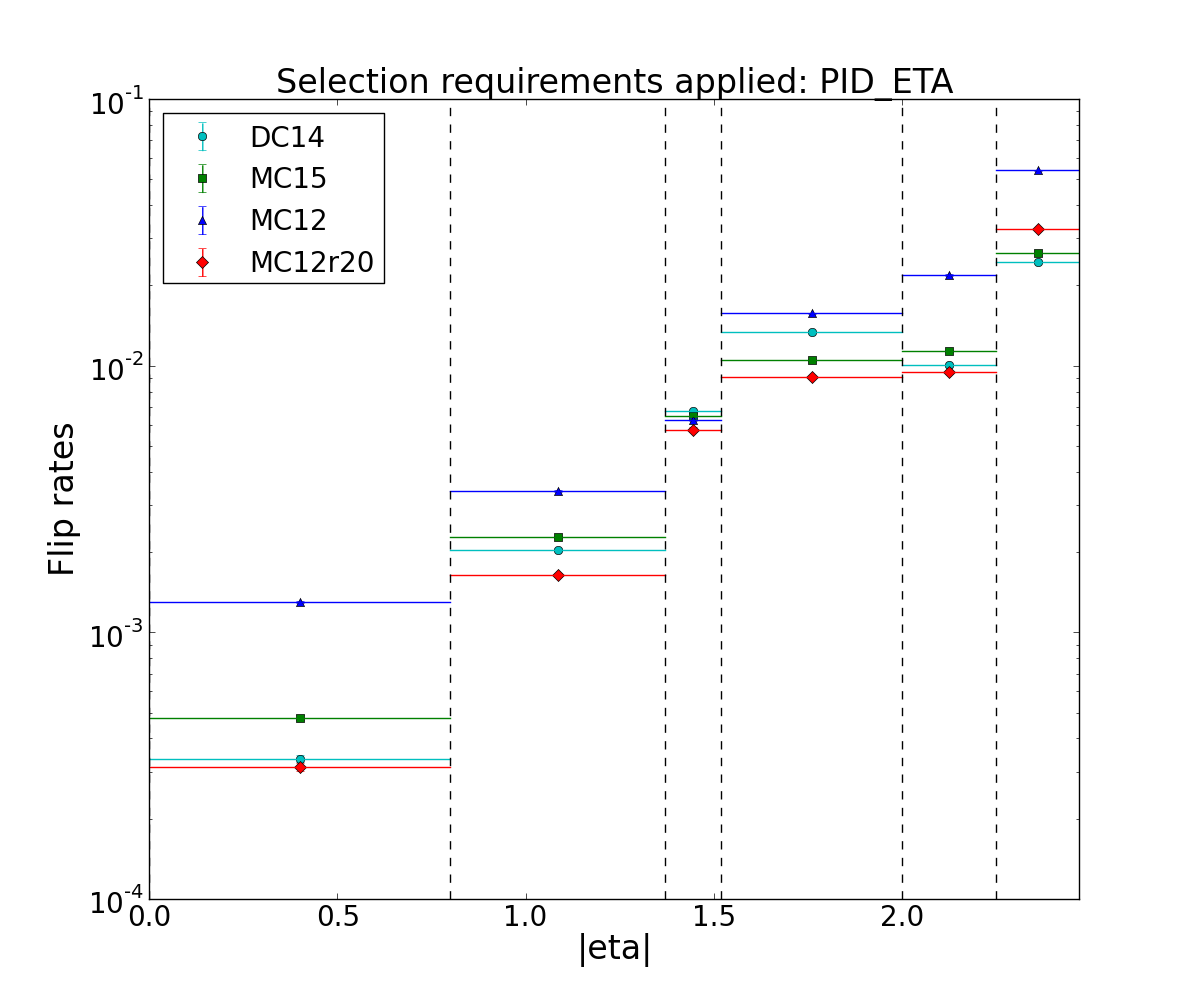
\includegraphics[width=0.4\linewidth]{FIGURES/BKG/chargeFlip/APPENDIX/fliprates_eta_PID_ETA.png}
\vfill
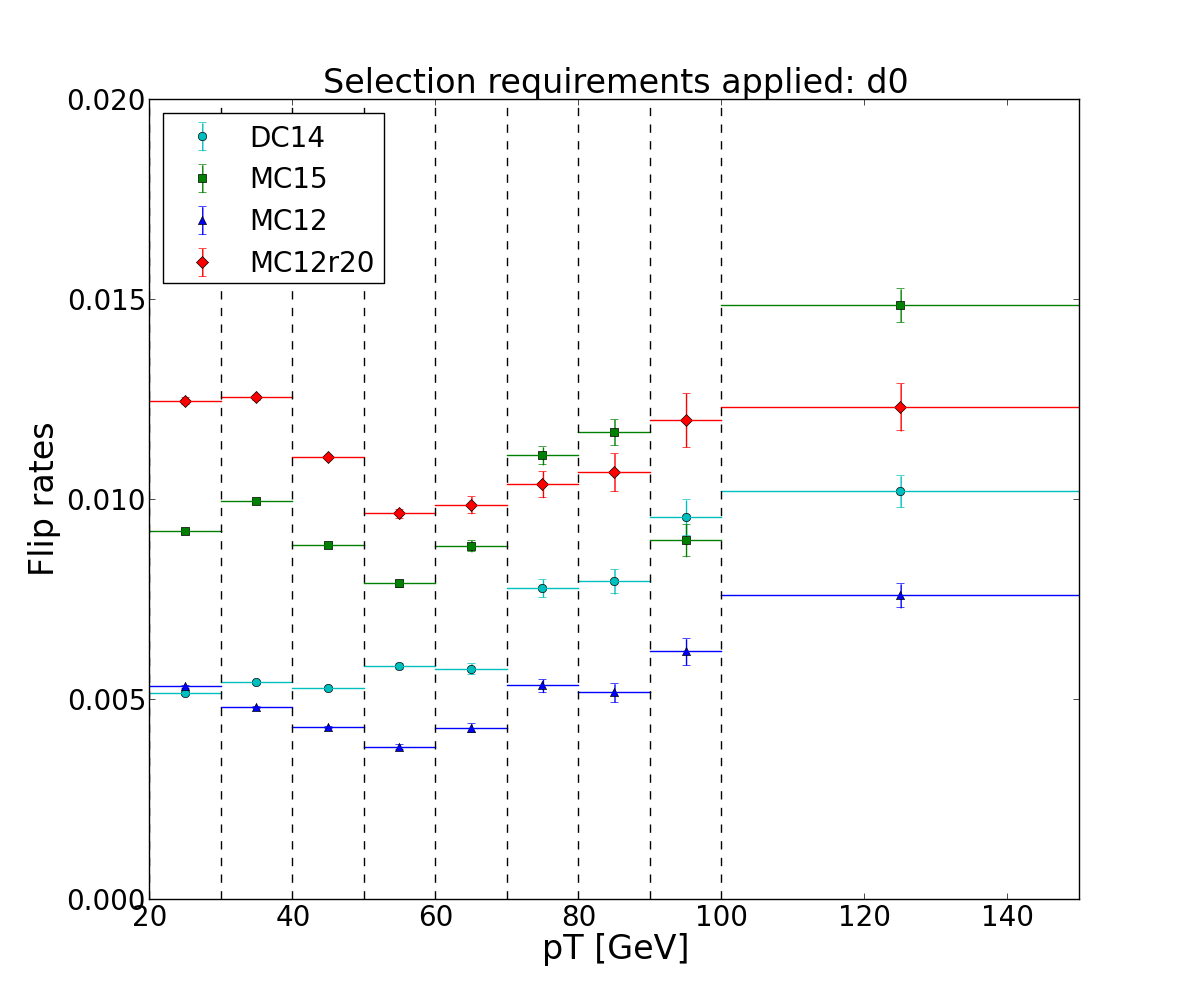
\includegraphics[width=0.4\linewidth]{FIGURES/BKG/chargeFlip/APPENDIX/fliprates_pT_d0.png}
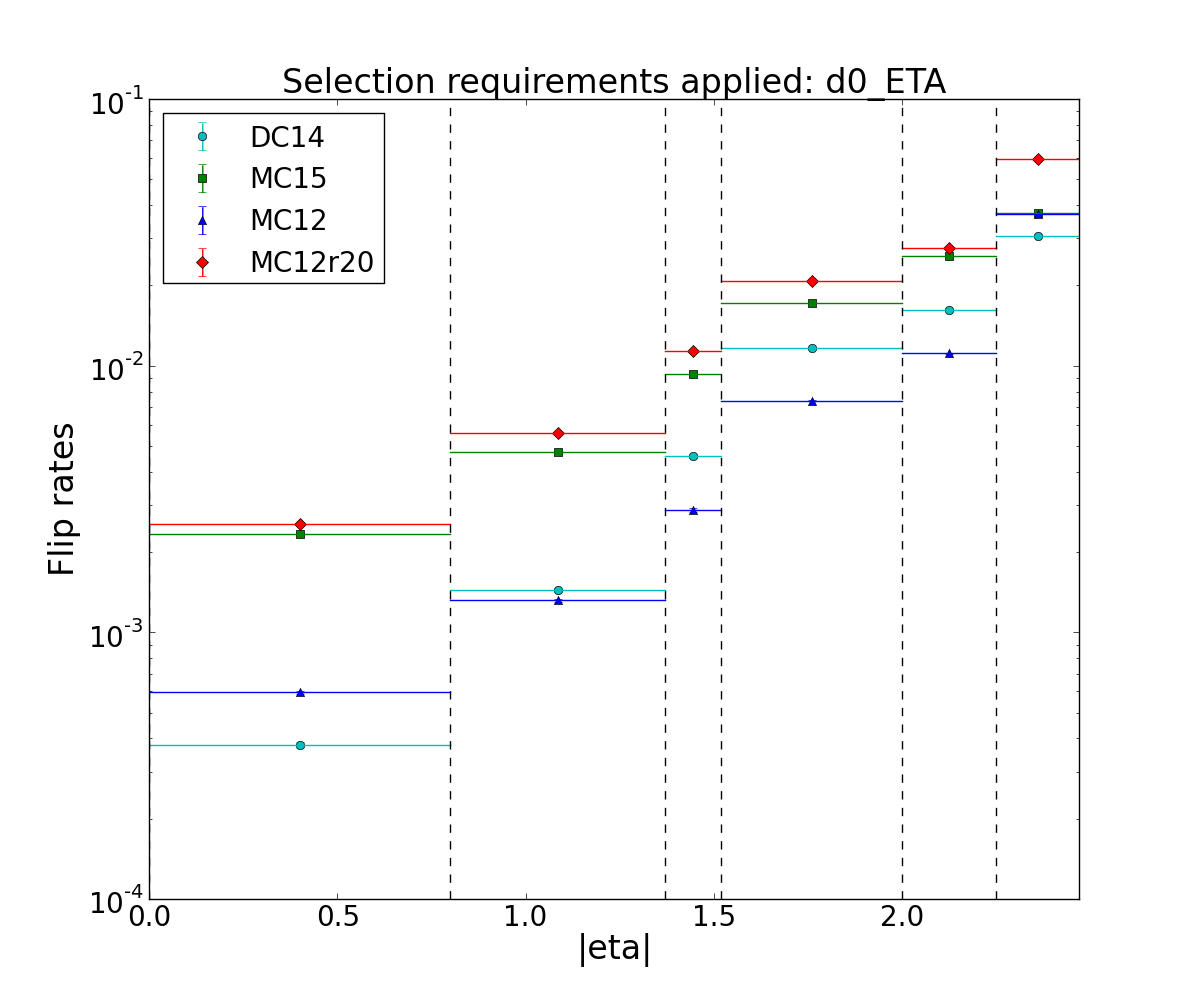
\includegraphics[width=0.4\linewidth]{FIGURES/BKG/chargeFlip/APPENDIX/fliprates_eta_d0_ETA.png}
\end{center}
\caption{\label{fig:all} Charge flip rates extracted from different MC samples with a $\pt$ binning for the left handed plots and with an $\eta$ binning for the right handed plots (only statistical uncertainties are shown). On the top plots, all the cuts presented in Table \ref{tab:signal} are considered as signal selection cuts, on the middle ones, only PID (\texttt{TightPP}  or \texttt{TightLLH}) and transverse momentum ($\pt>20$ GeV) cuts are considered as signal selection cuts and on the bottom plots only transverse impact parameter ($\left | d_0 / \sigma(d_0) \right |<3.0$) and transverse momentum ($\pt>20$ GeV) cuts considered as signal selection cuts.}
\end{figure}
%------------------------------------------------

Figure~\ref{fig:nosigd0} shows the charge flip rates extracted again for different MC samples and with all signal selection cuts applied except the $d_0$ significance in order to understand in a better way its influence on the rates. The feature at low $\pt$ for MC12 sample is still present, meaning that the $d_0$ significance cut could be the one that compensate the effect coming from the PID requirements (shown on the middle left plot of Fig. \ref{fig:all}). Furthermore, the MC12 and MC15 charge flip rates are closer to each other in comparison of the distribution shown on the top left plot in Fig. \ref{fig:all}. This comparison shows again that cutting or not on the $d_0$ significance have a large impact on the disagreement between charge flip rates coming from MC12 and MC15 results. This study is still ongoing and one of the main future hypothesis is that the $d_0$ definitions used in MC12 and MC15 samples are not the same: $d_0$ could be defined with respect to the primary vertex in MC12 sample and with respect to the beam spot in MC15. Nevertheless, this study has shown that the charge mis-measurement rates were increased between the old MC12 samples used in Run 1 and the new MC15 samples used during Run 2.

%------------------------------------------------
\begin{figure}[htb!]
\centering
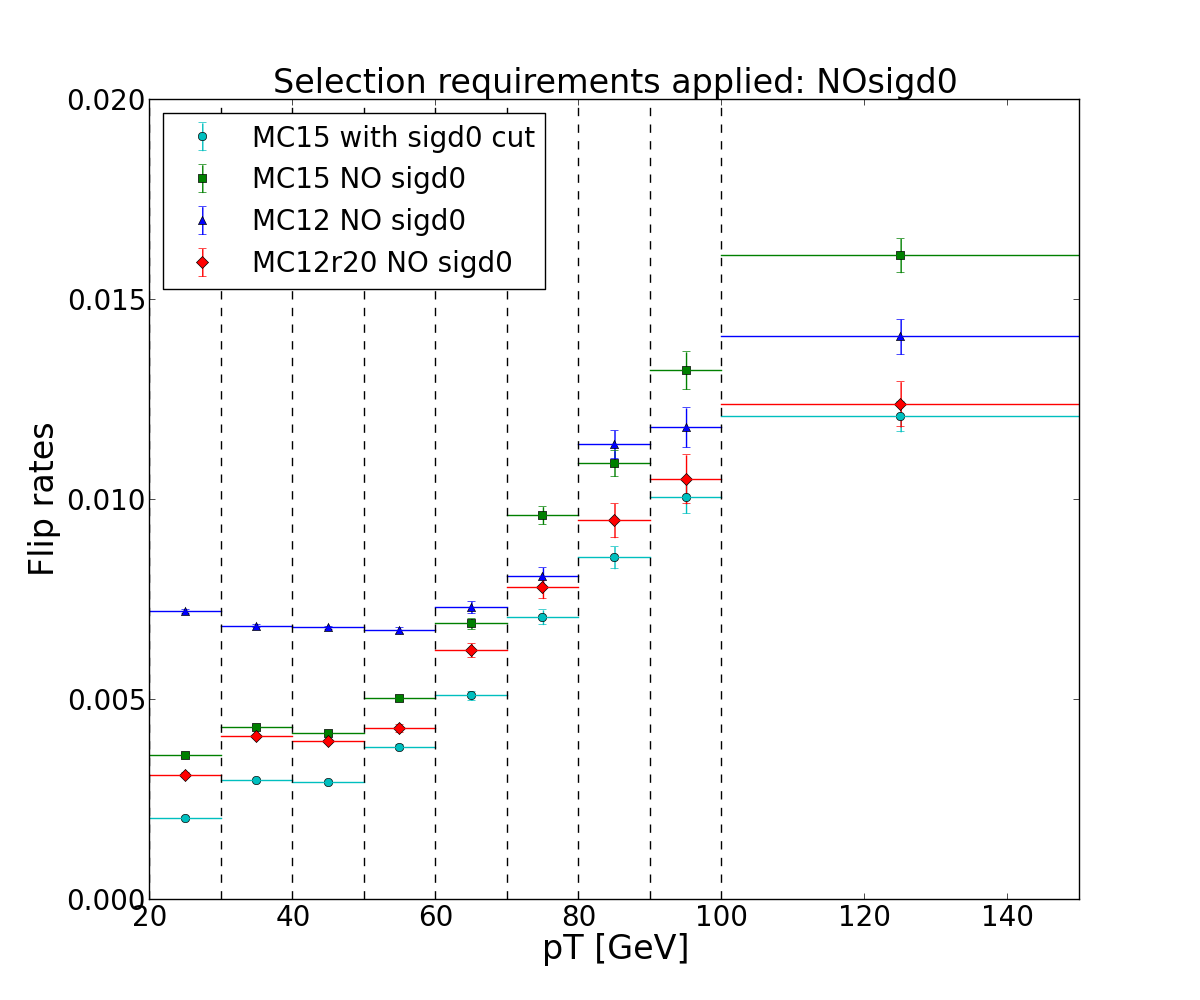
\includegraphics[width=0.5\linewidth]{FIGURES/BKG/chargeFlip/APPENDIX/fliprates_pT_NOsigd0.png}
\caption{\label{fig:nosigd0} Charge flip rates extracted from different MC samples with a $\pt$ binning and for the case where all signal selections cuts  from Table \ref{tab:signal} are applied except the $d_0$ significance cut (only statistical uncertainties are shown).}
\end{figure}
%------------------------------------------------


\FloatBarrier

\subsection{Charge flip rates plots: MC12 vs. DC14 vs. MC15}
\label{app:CFrates1}

\begin{figure}[!htbp]
\centering
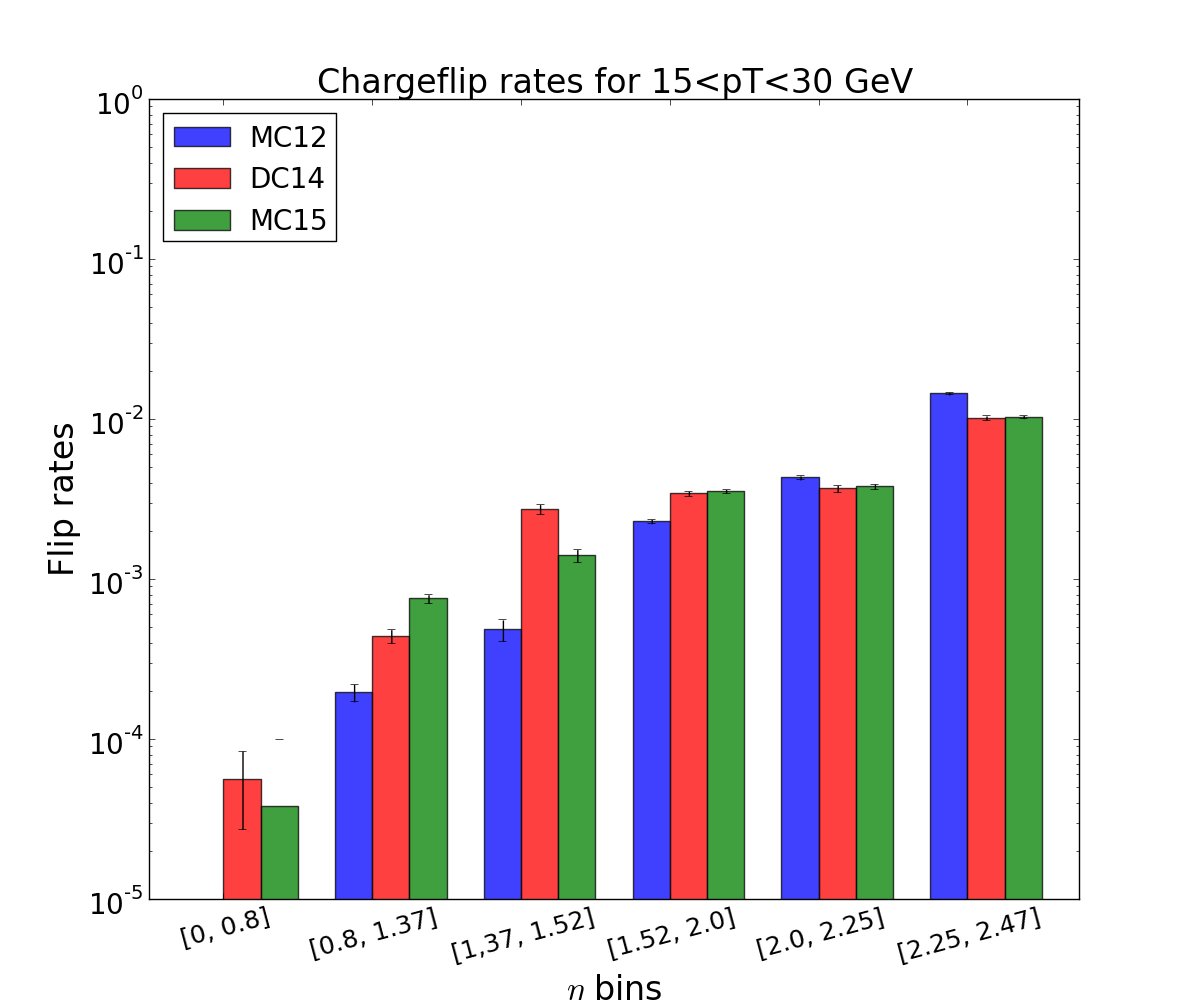
\includegraphics[width=0.33\linewidth]{FIGURES/BKG/chargeFlip/APPENDIX/fliprates_MC12/fliprates_3samples_15.png}
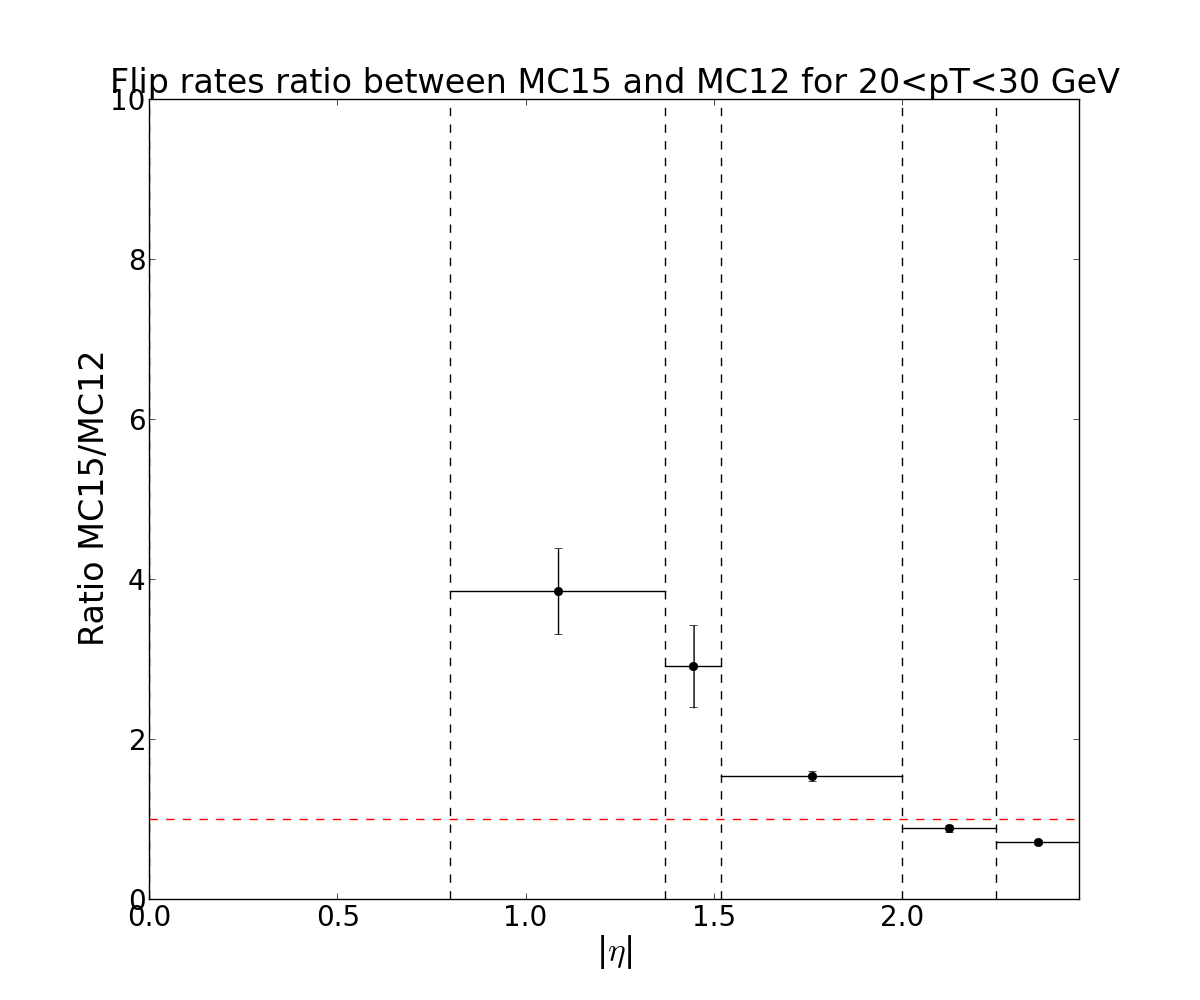
\includegraphics[width=0.33\linewidth]{FIGURES/BKG/chargeFlip/APPENDIX/ratio_MC15vsMC12/ratio_plot_20.png}
\vfill
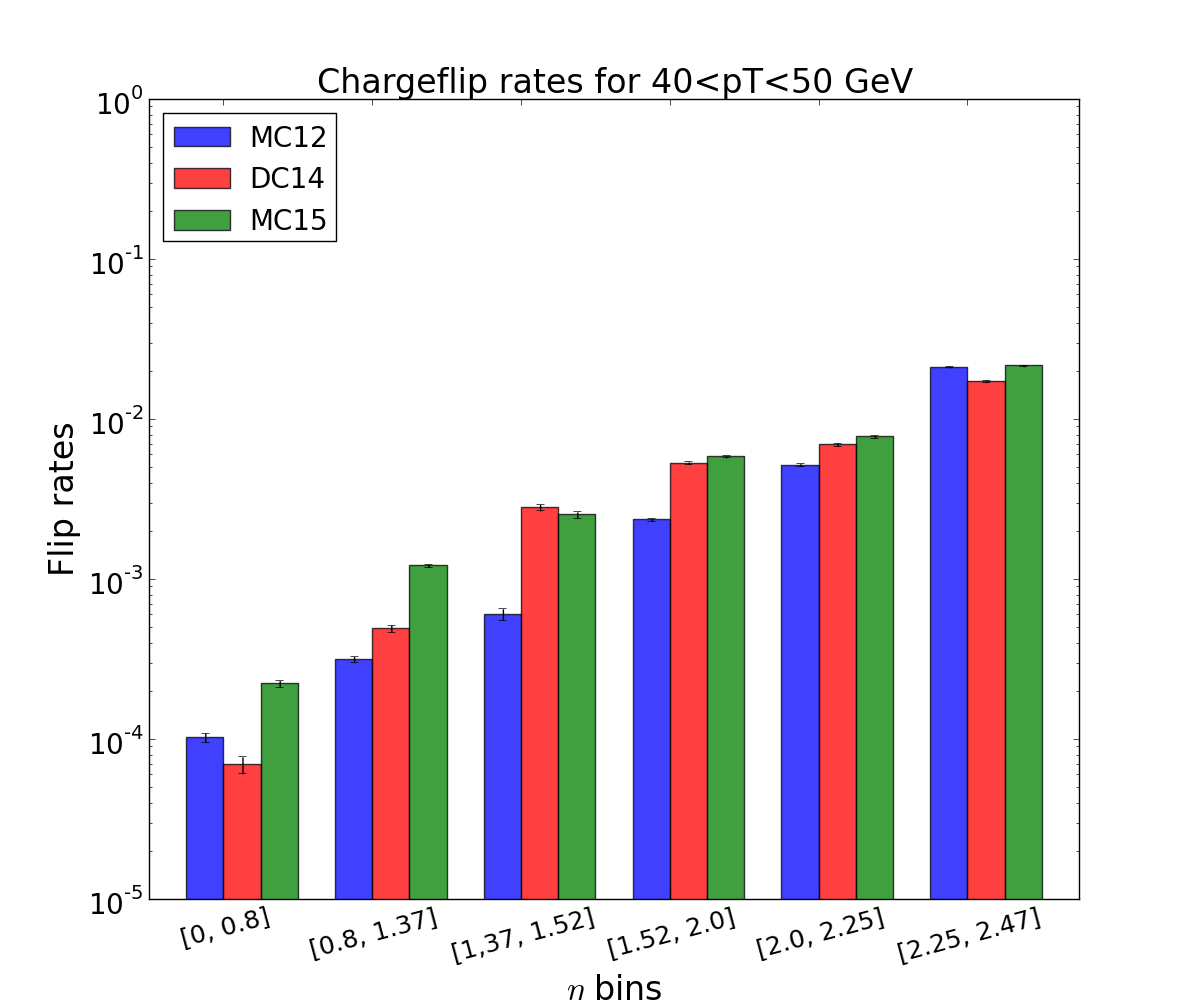
\includegraphics[width=0.33\linewidth]{FIGURES/BKG/chargeFlip/APPENDIX/fliprates_MC12/fliprates_3samples_40.png}
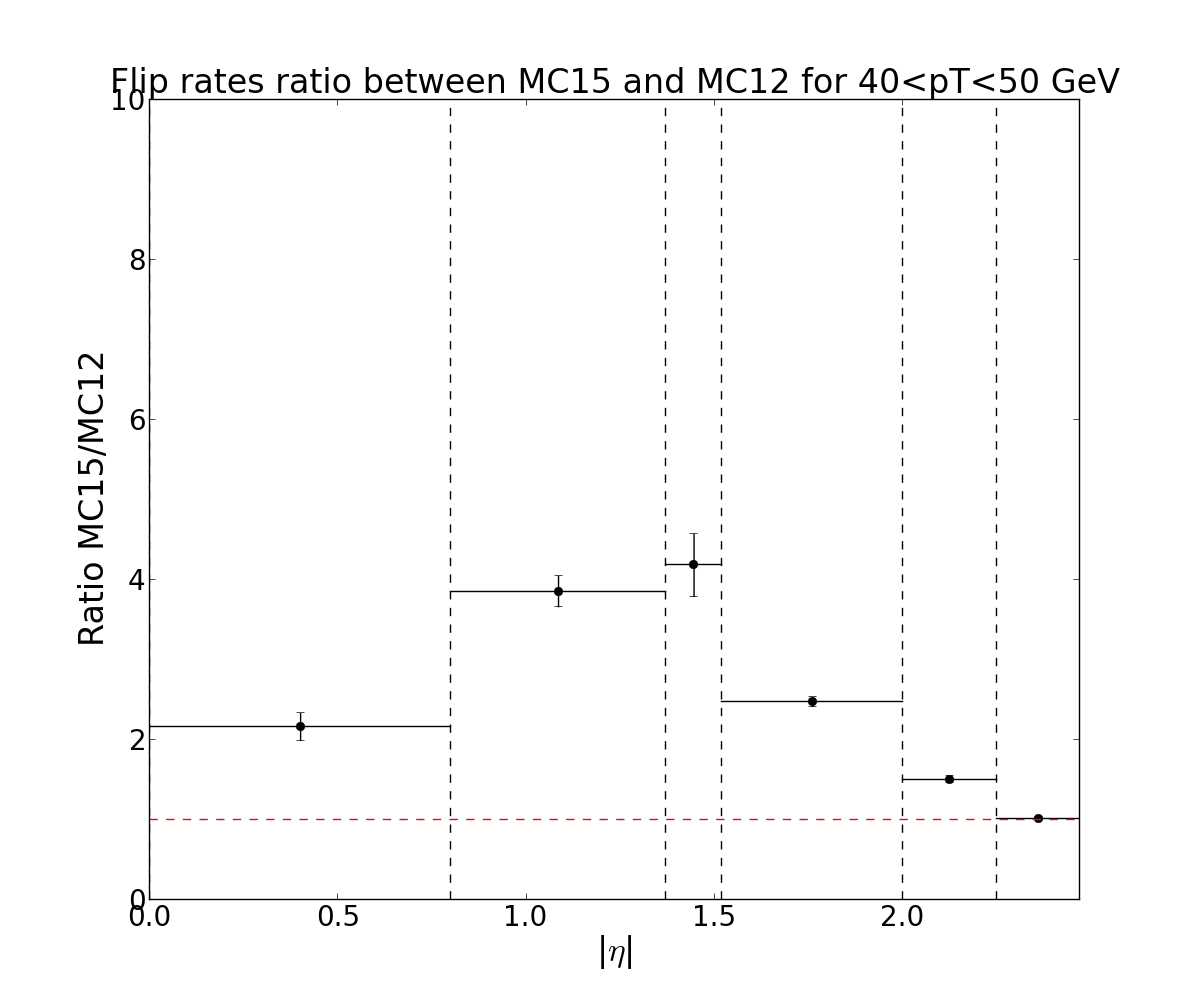
\includegraphics[width=0.33\linewidth]{FIGURES/BKG/chargeFlip/APPENDIX/ratio_MC15vsMC12/ratio_plot_40.png}
\vfill
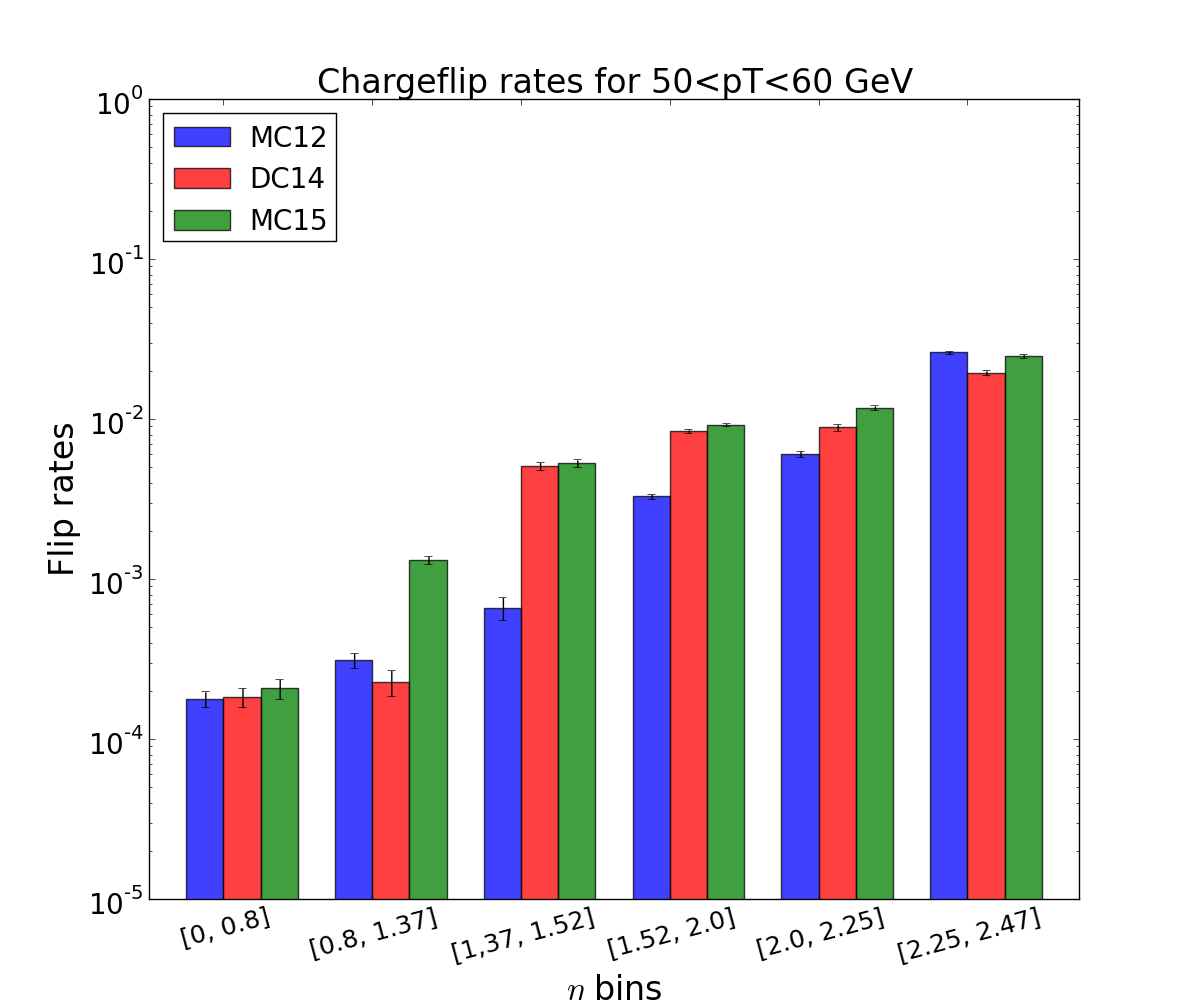
\includegraphics[width=0.33\linewidth]{FIGURES/BKG/chargeFlip/APPENDIX/fliprates_MC12/fliprates_3samples_50.png}
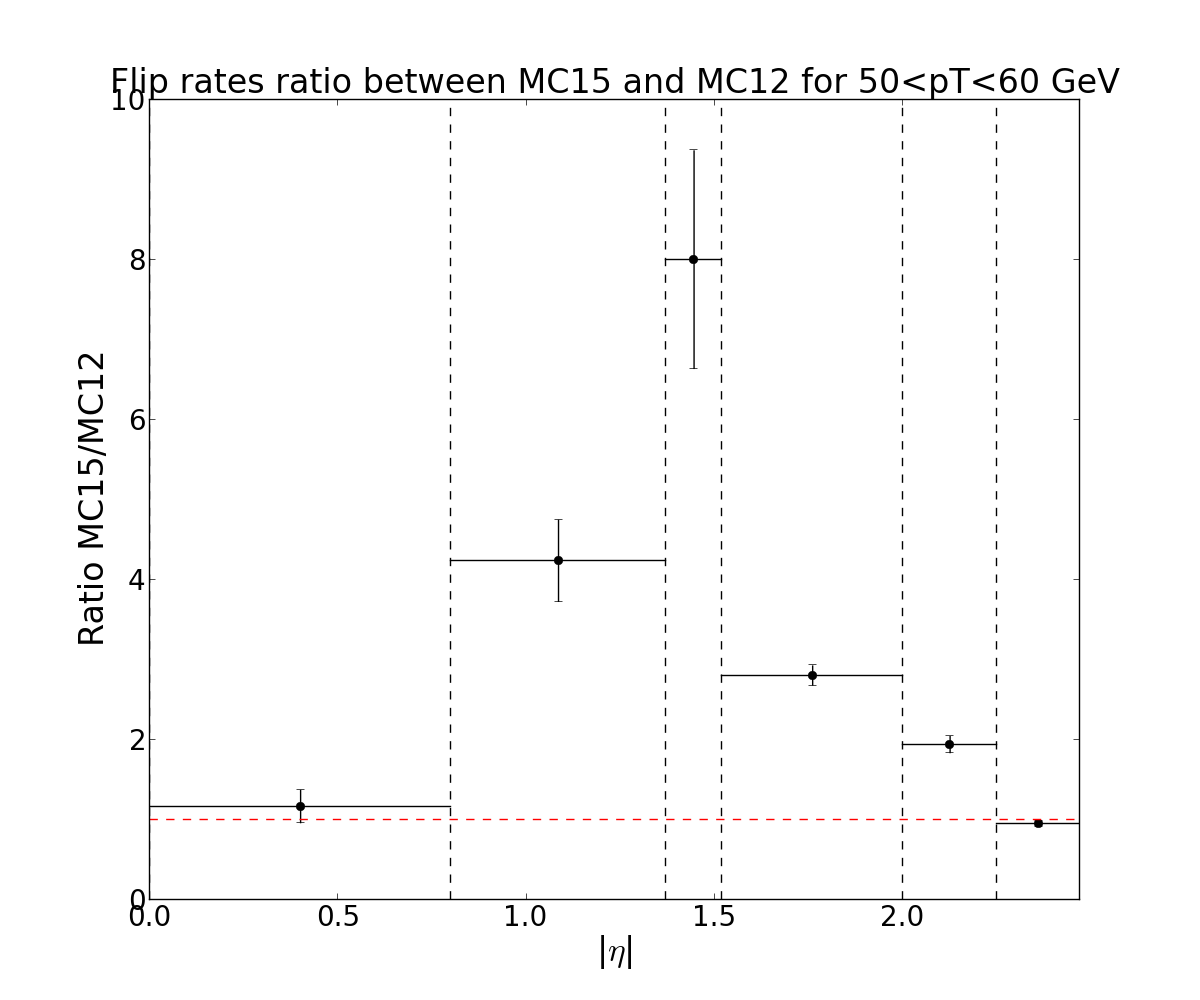
\includegraphics[width=0.33\linewidth]{FIGURES/BKG/chargeFlip/APPENDIX/ratio_MC15vsMC12/ratio_plot_50.png}
\vfill
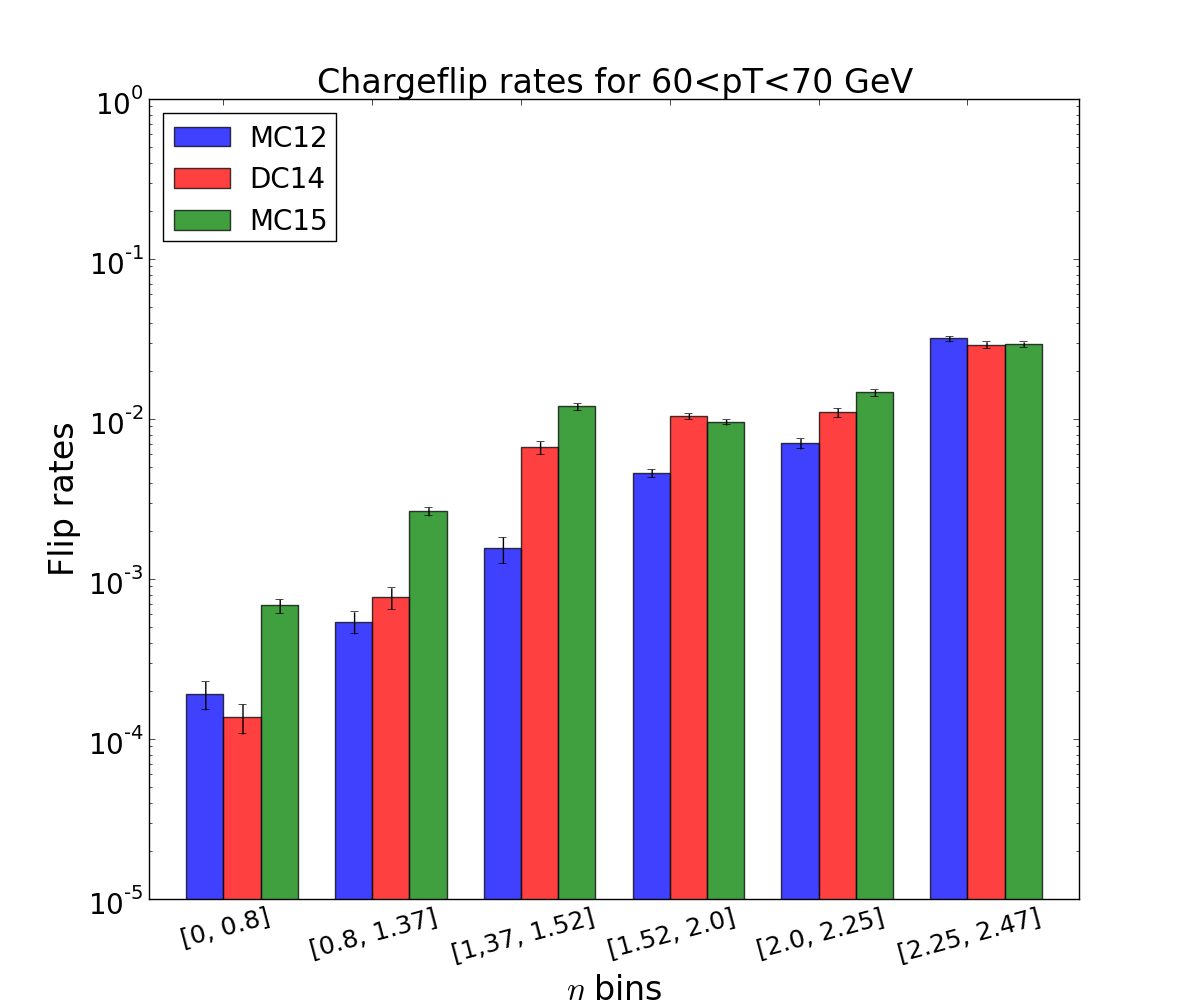
\includegraphics[width=0.33\linewidth]{FIGURES/BKG/chargeFlip/APPENDIX/fliprates_MC12/fliprates_3samples_60.png}
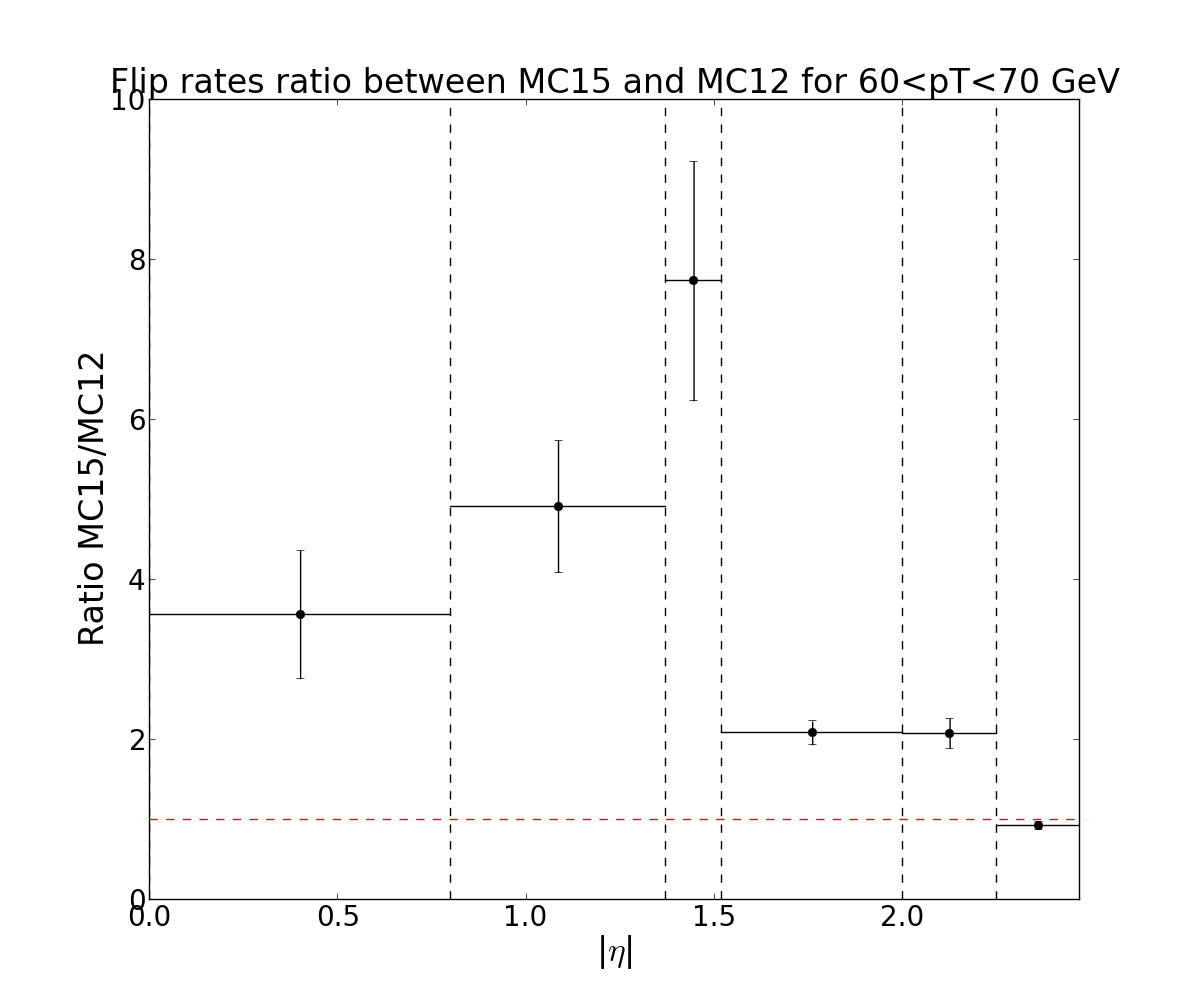
\includegraphics[width=0.33\linewidth]{FIGURES/BKG/chargeFlip/APPENDIX/ratio_MC15vsMC12/ratio_plot_60.png}
\caption{\label{fig:12vs15_2030} On the left, charge flip rates extracted from MC12 sample in blue, DC14 sample in red and MC15 in green. On the right, ratios between MC15 and MC12 charge flip rates. Only statistical uncertainties are shown. The rates and ratios are computed for 6 different $\eta$ bins and one $\pt$ bin (from top-to bottom): $20<\pt<30$ GeV, $40<\pt<50$ GeV, $50<\pt<60$ GeV, $60<\pt<70$ GeV.}
\end{figure}

\begin{figure}[!htbp]
\centering
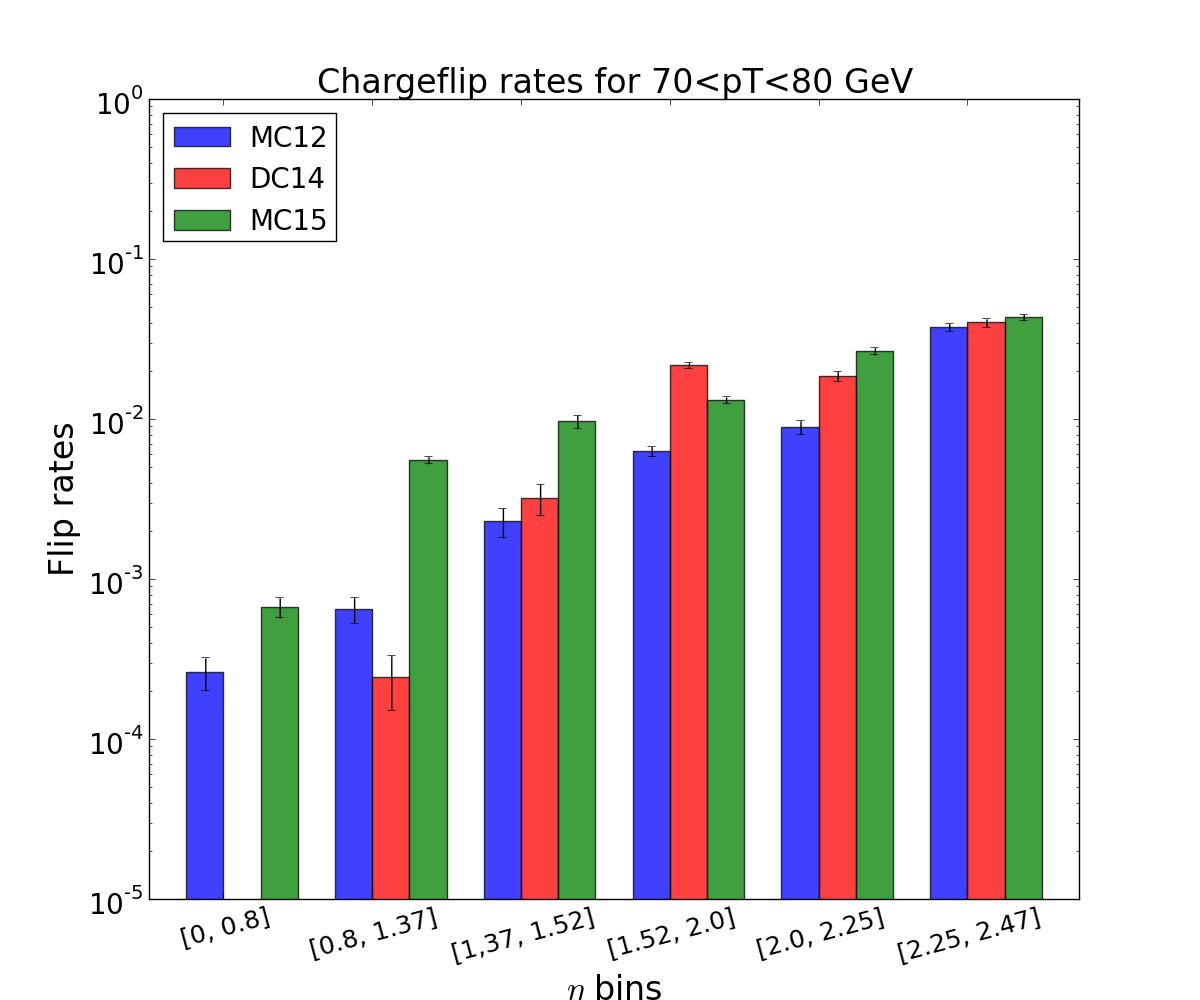
\includegraphics[width=0.33\linewidth]{FIGURES/BKG/chargeFlip/APPENDIX/fliprates_MC12/fliprates_3samples_70.png}
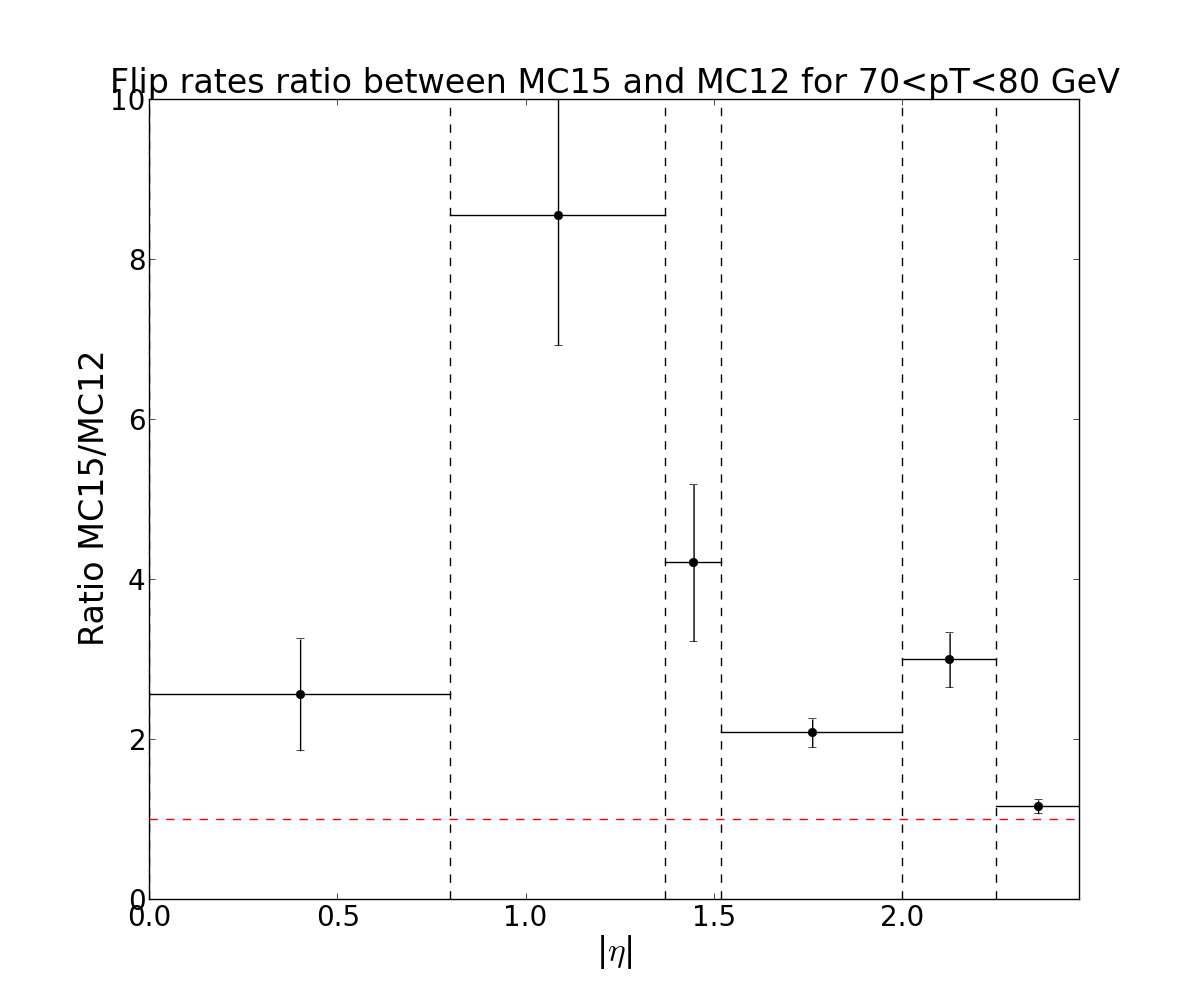
\includegraphics[width=0.33\linewidth]{FIGURES/BKG/chargeFlip/APPENDIX/ratio_MC15vsMC12/ratio_plot_70.png}
\vfill
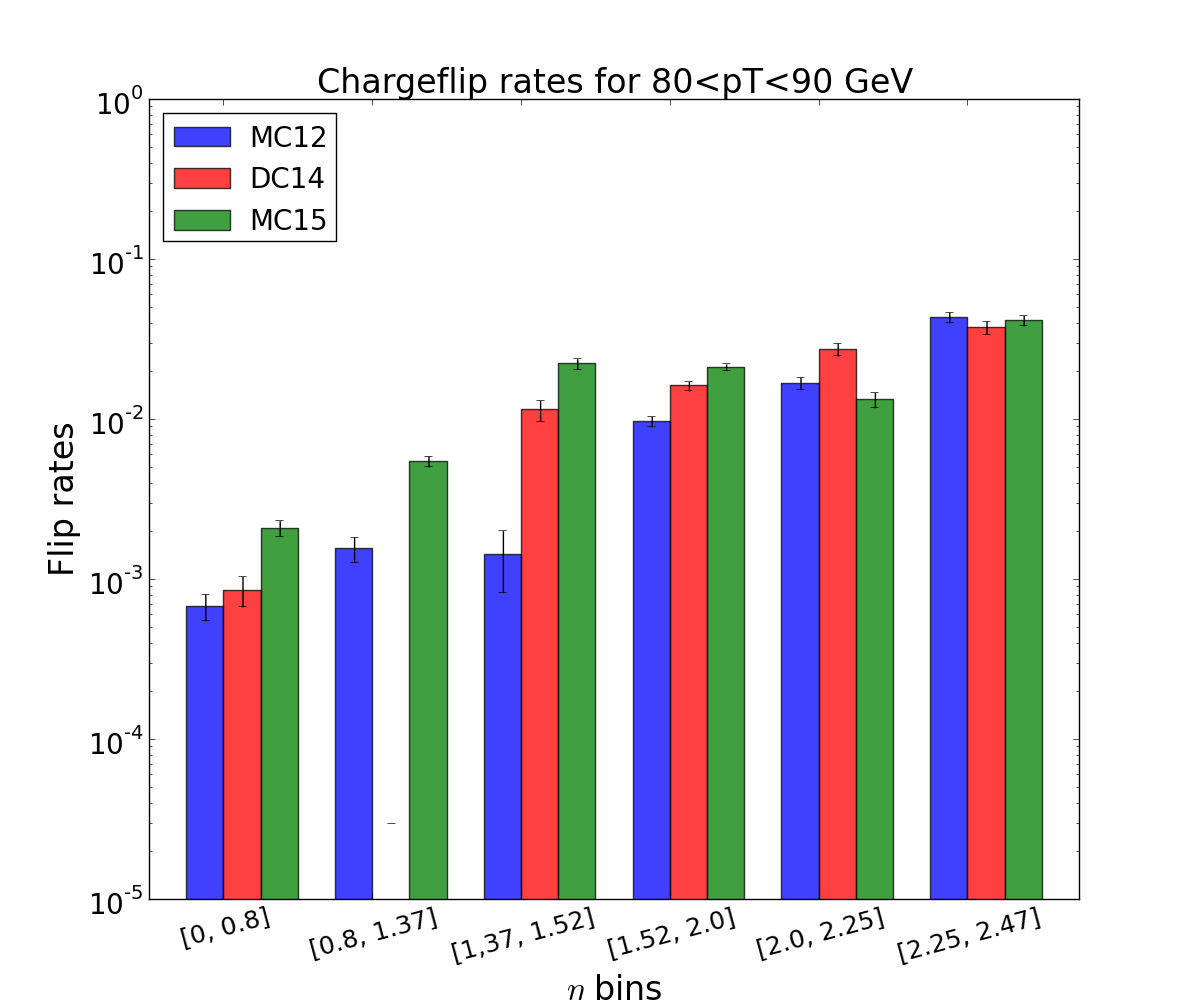
\includegraphics[width=0.33\linewidth]{FIGURES/BKG/chargeFlip/APPENDIX/fliprates_MC12/fliprates_3samples_80.png}
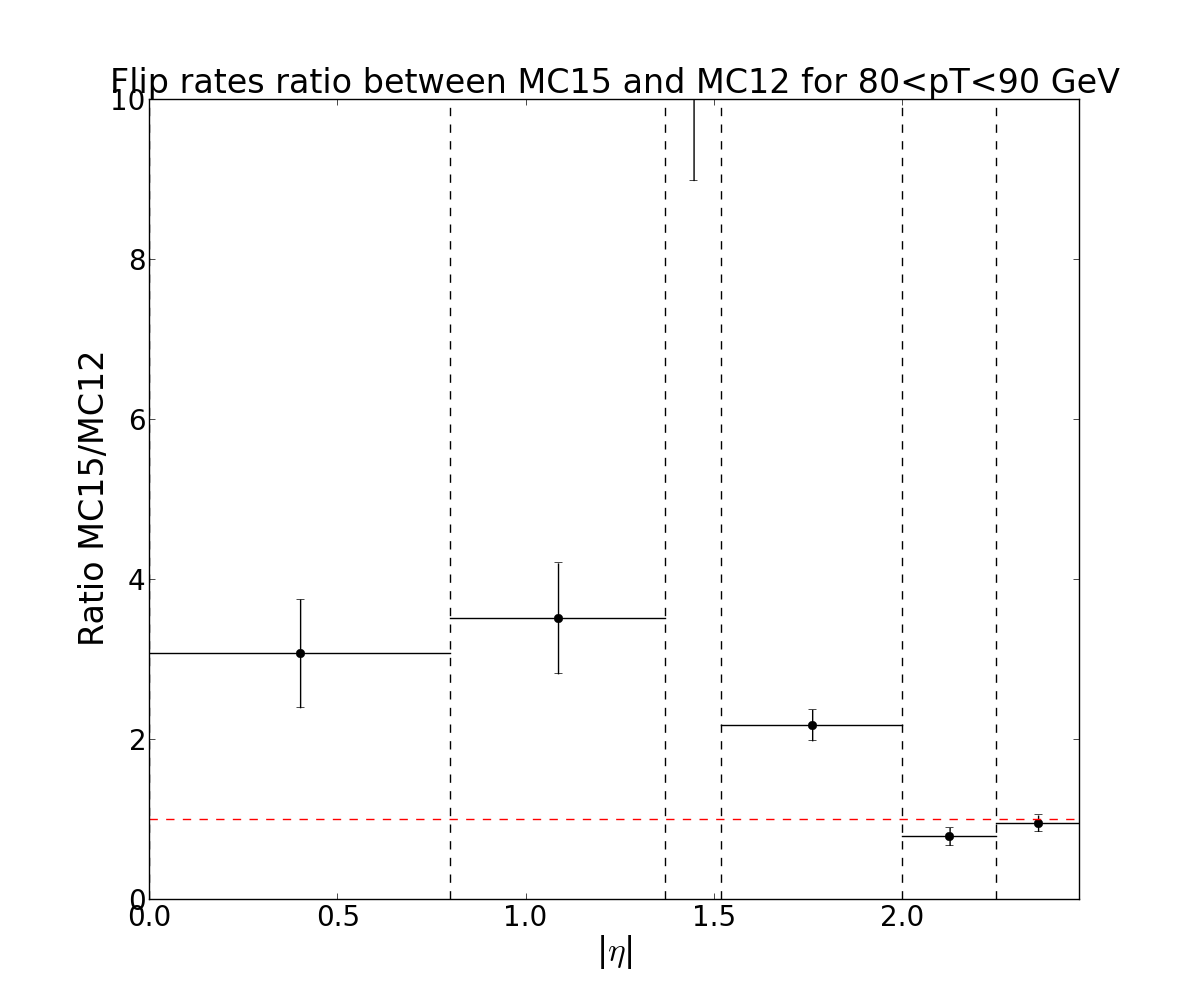
\includegraphics[width=0.33\linewidth]{FIGURES/BKG/chargeFlip/APPENDIX/ratio_MC15vsMC12/ratio_plot_80.png}
\vfill
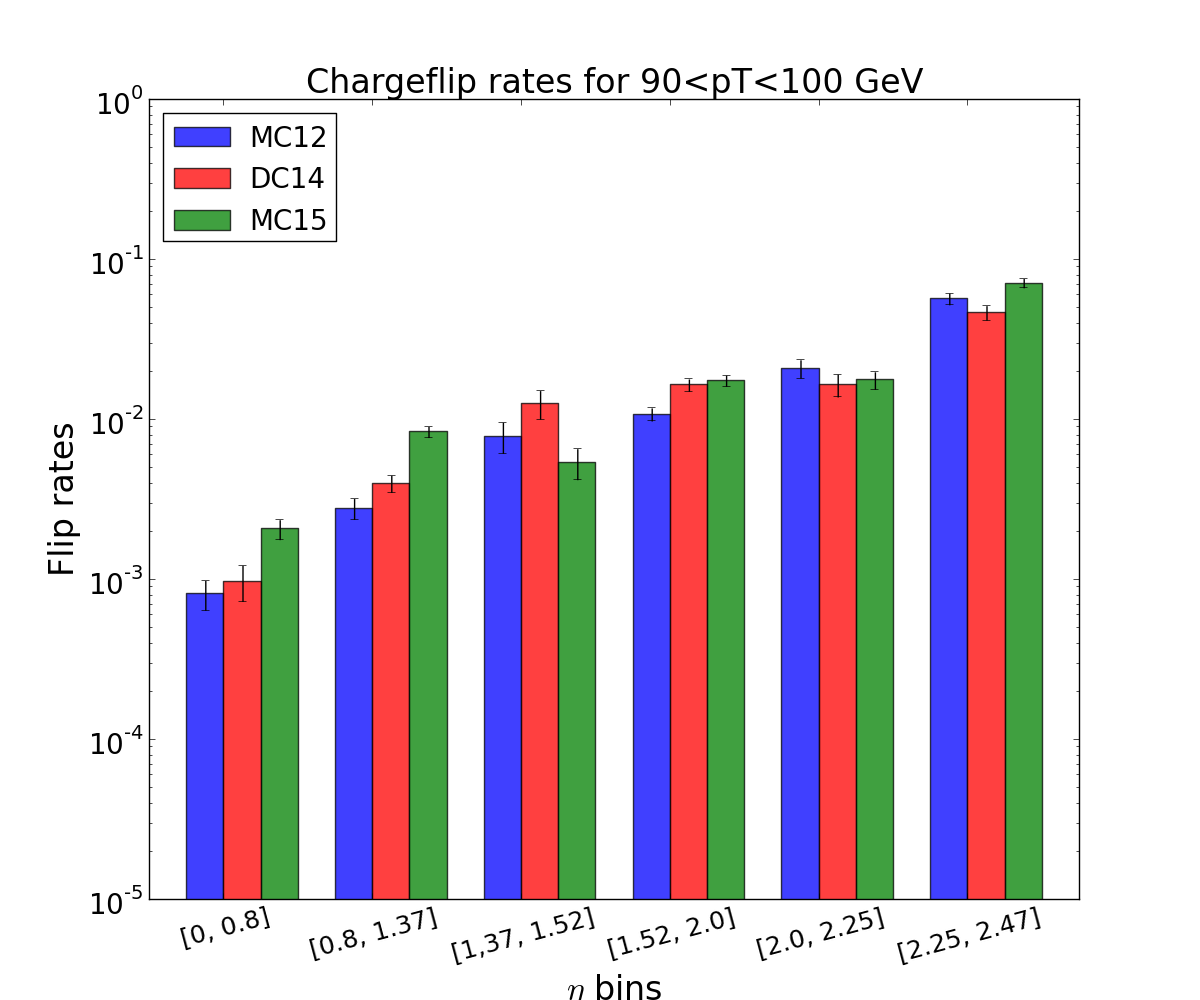
\includegraphics[width=0.33\linewidth]{FIGURES/BKG/chargeFlip/APPENDIX/fliprates_MC12/fliprates_3samples_90.png}
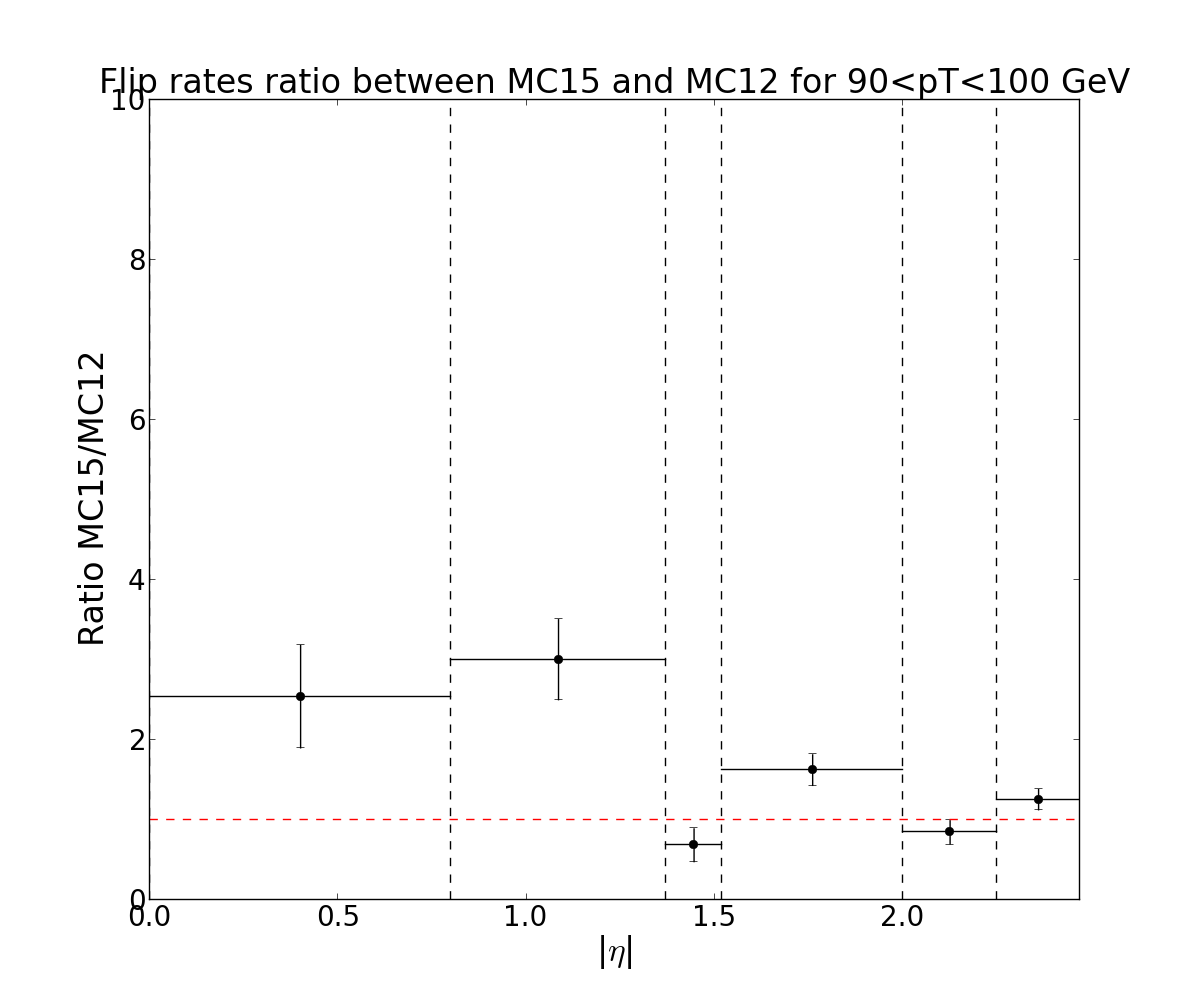
\includegraphics[width=0.33\linewidth]{FIGURES/BKG/chargeFlip/APPENDIX/ratio_MC15vsMC12/ratio_plot_90.png}
\vfill
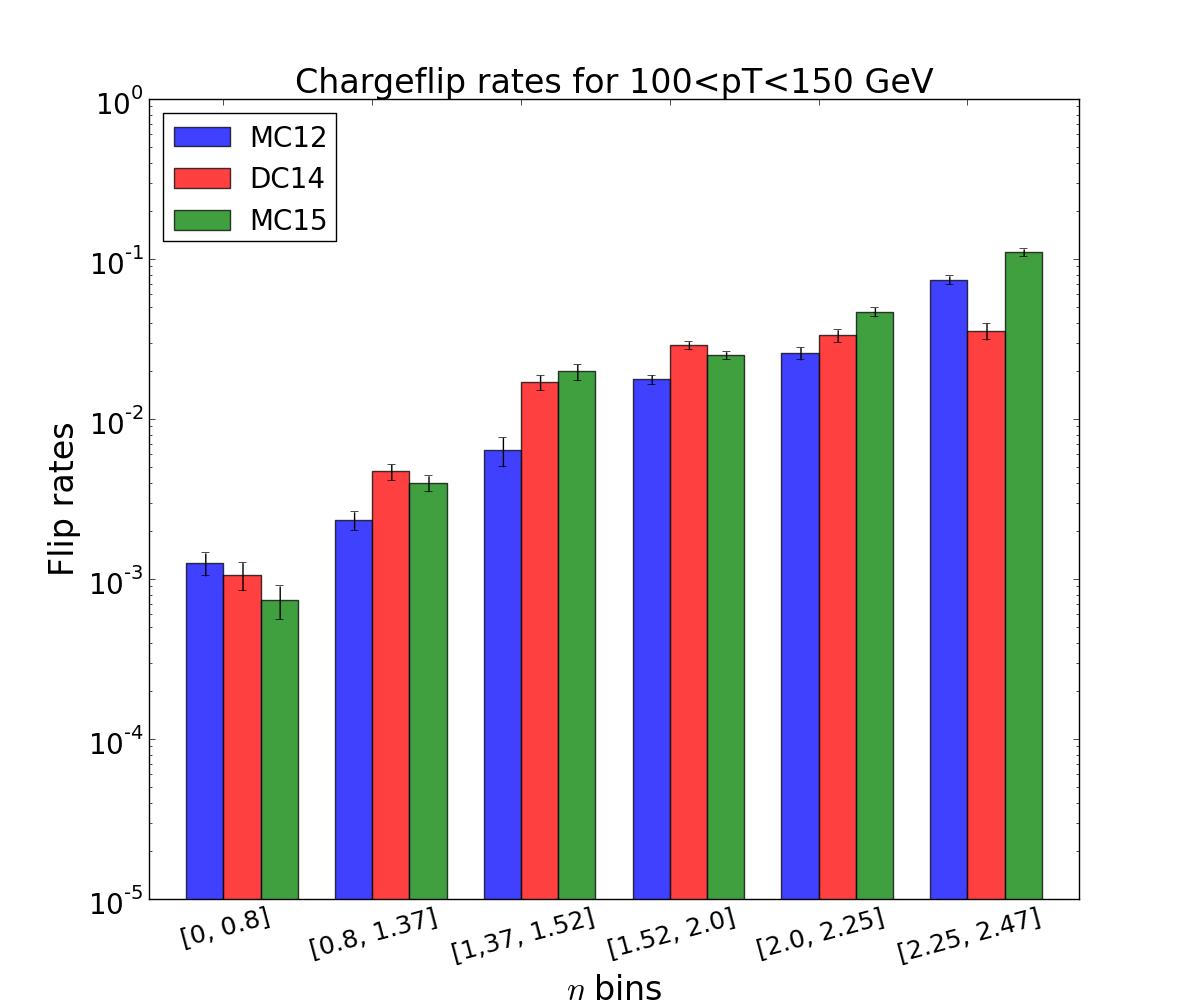
\includegraphics[width=0.33\linewidth]{FIGURES/BKG/chargeFlip/APPENDIX/fliprates_MC12/fliprates_3samples_100.png}
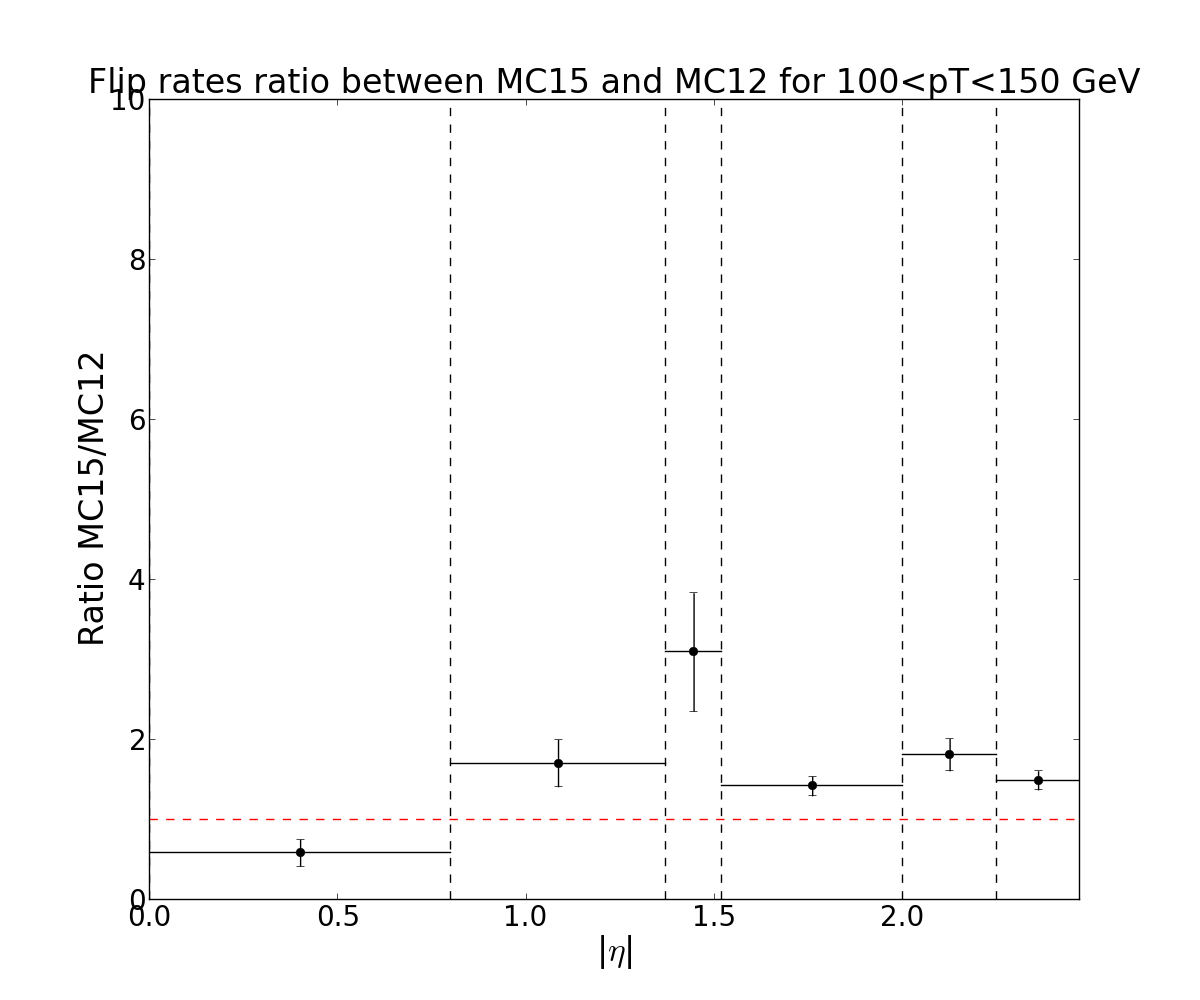
\includegraphics[width=0.33\linewidth]{FIGURES/BKG/chargeFlip/APPENDIX/ratio_MC15vsMC12/ratio_plot_100.png}
\caption{\label{fig:12vs15_7080} On the left, charge flip rates extracted from MC12 sample in blue, DC14 sample in red and MC15 in green. On the right, ratios between MC15 and MC12 charge flip rates. Only statistical uncertainties are shown. The rates and ratios are computed for 6 different $\eta$ bins and one $\pt$ bin (from top-to bottom): $70<\pt<80$ GeV, $80<\pt<90$ GeV, $90<\pt<100$ GeV, $100<\pt<150$ GeV.}
\end{figure}

\FloatBarrier

\subsection{Charge flip rates plots: MC12 vs. MC15 vs. MC12r20}
\label{app:CFrates2}

\begin{figure}[!htbp]
\centering
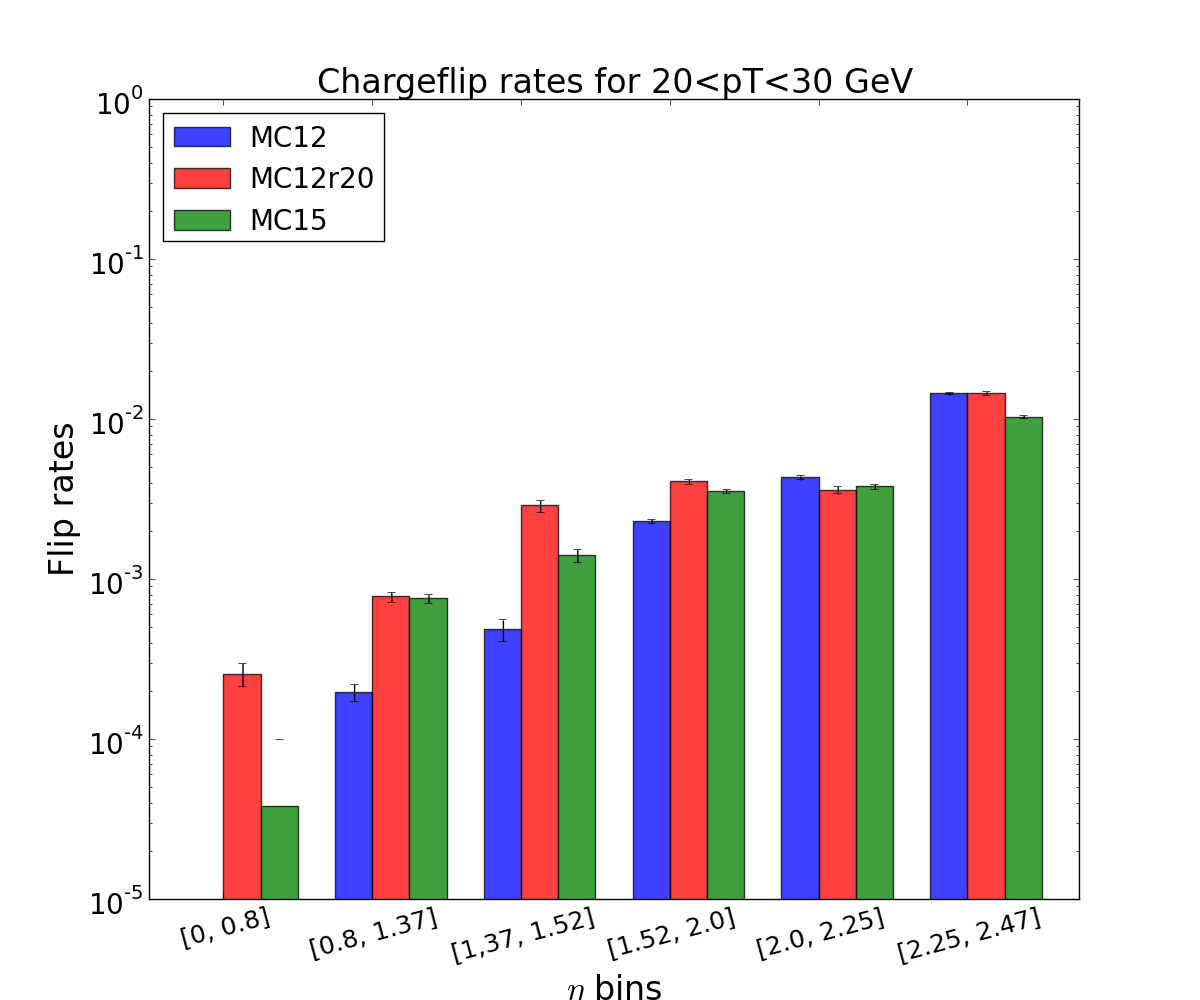
\includegraphics[width=0.33\linewidth]{FIGURES/BKG/chargeFlip/APPENDIX/fliprates_MC12r20/fliprates_3samples_20.png}
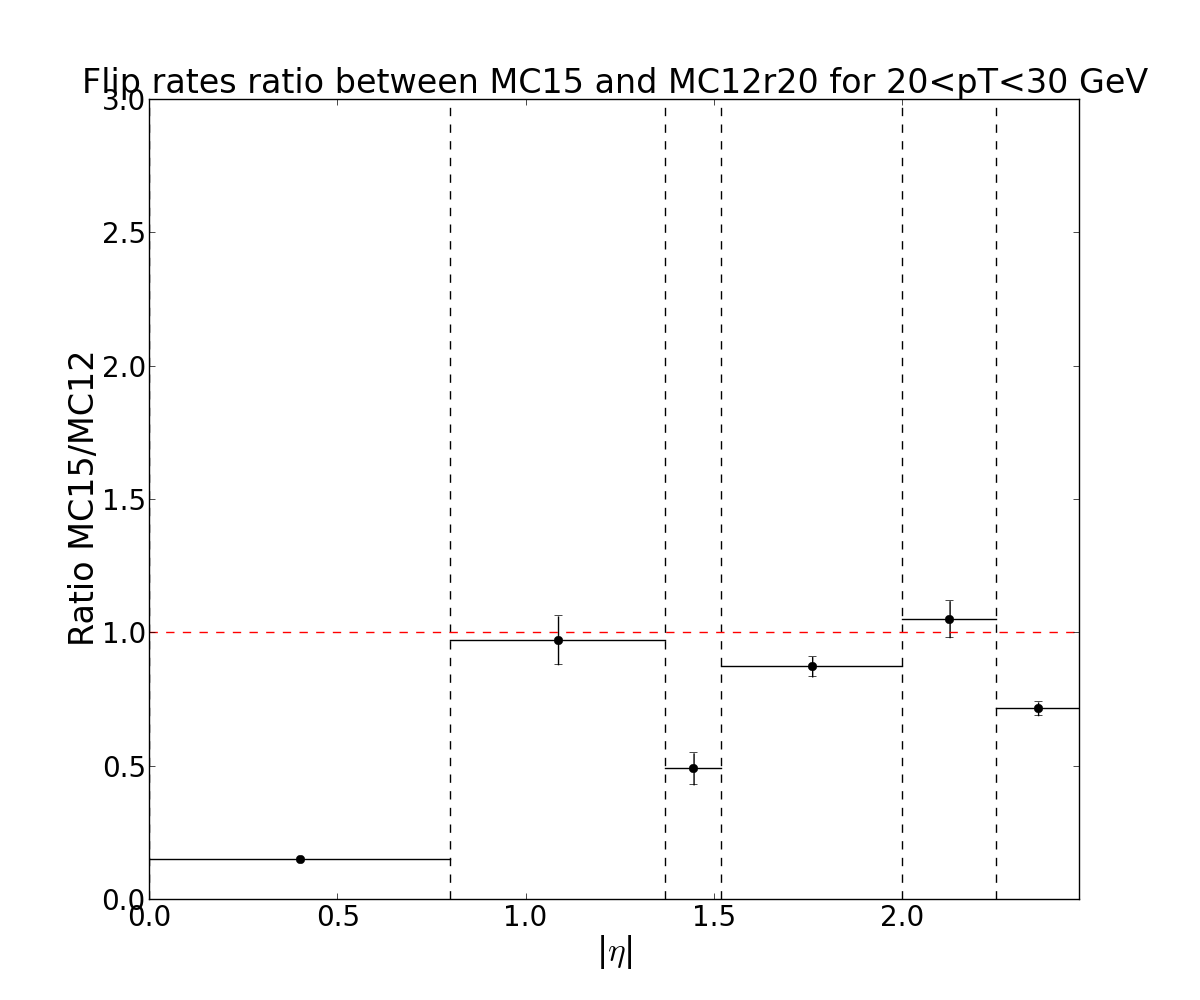
\includegraphics[width=0.33\linewidth]{FIGURES/BKG/chargeFlip/APPENDIX/ratio_MC15vsMC12r20/ratio_plot_20.png}
\vfill
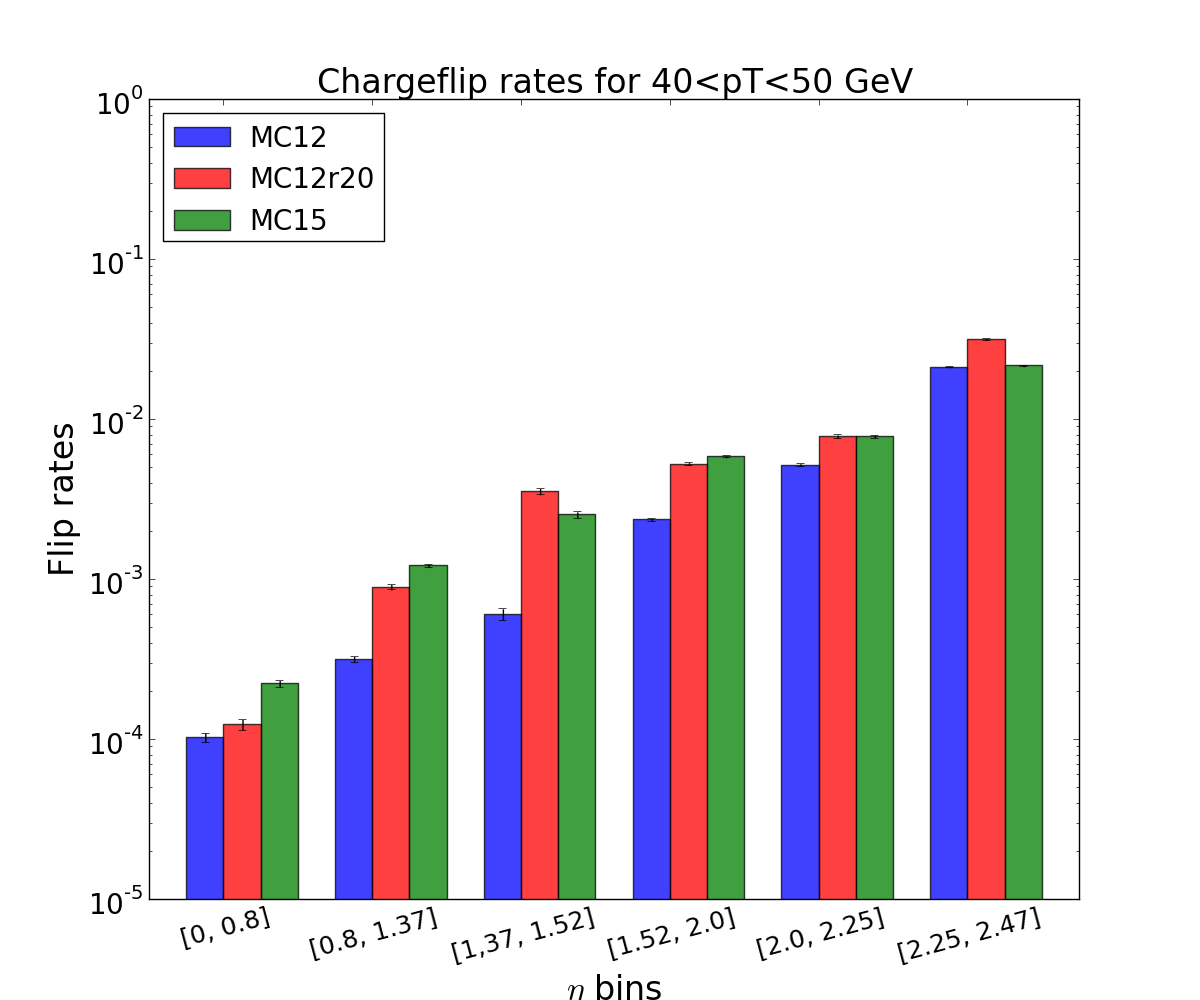
\includegraphics[width=0.33\linewidth]{FIGURES/BKG/chargeFlip/APPENDIX/fliprates_MC12r20/fliprates_3samples_40.png}
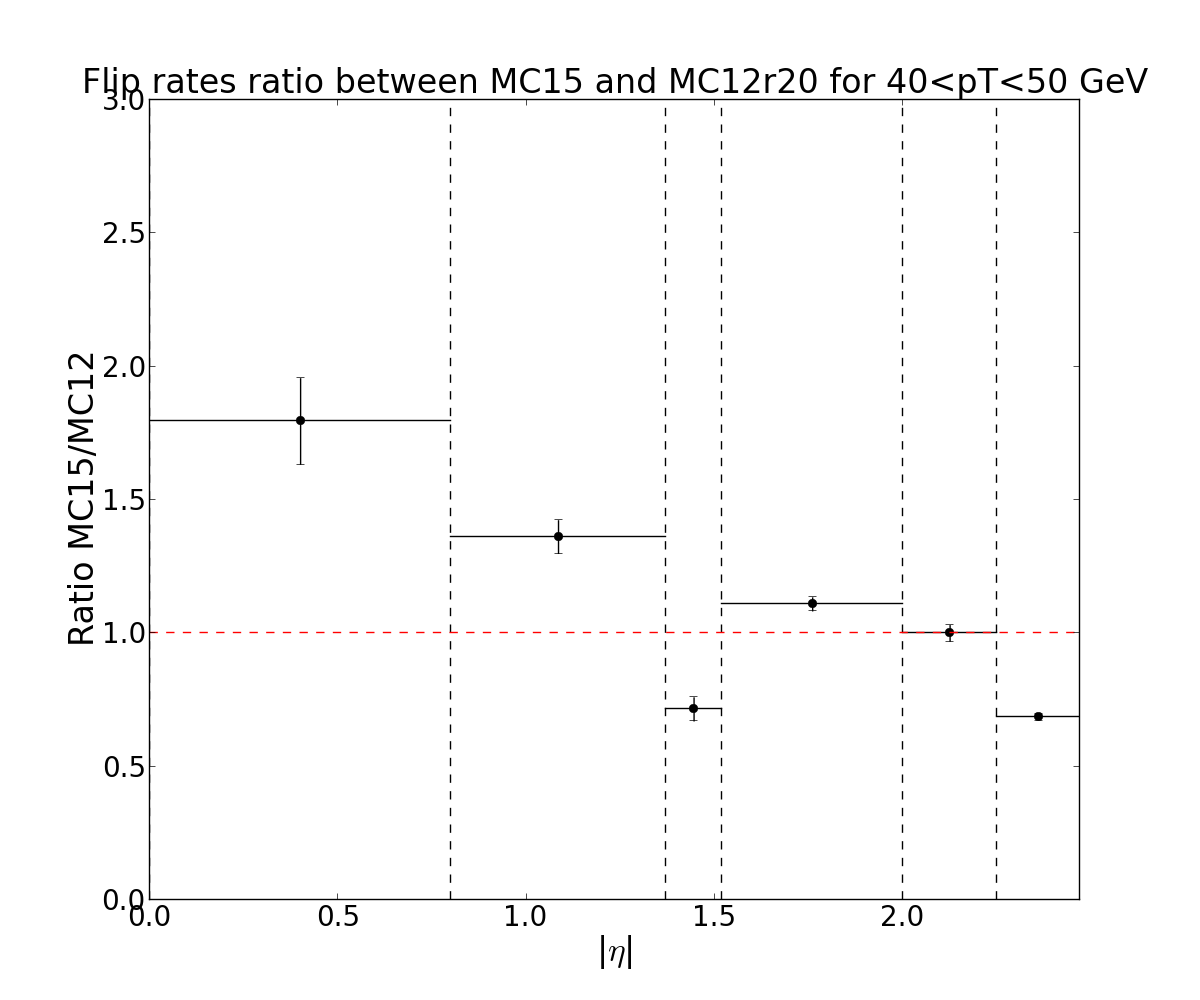
\includegraphics[width=0.33\linewidth]{FIGURES/BKG/chargeFlip/APPENDIX/ratio_MC15vsMC12r20/ratio_plot_40.png}
\vfill
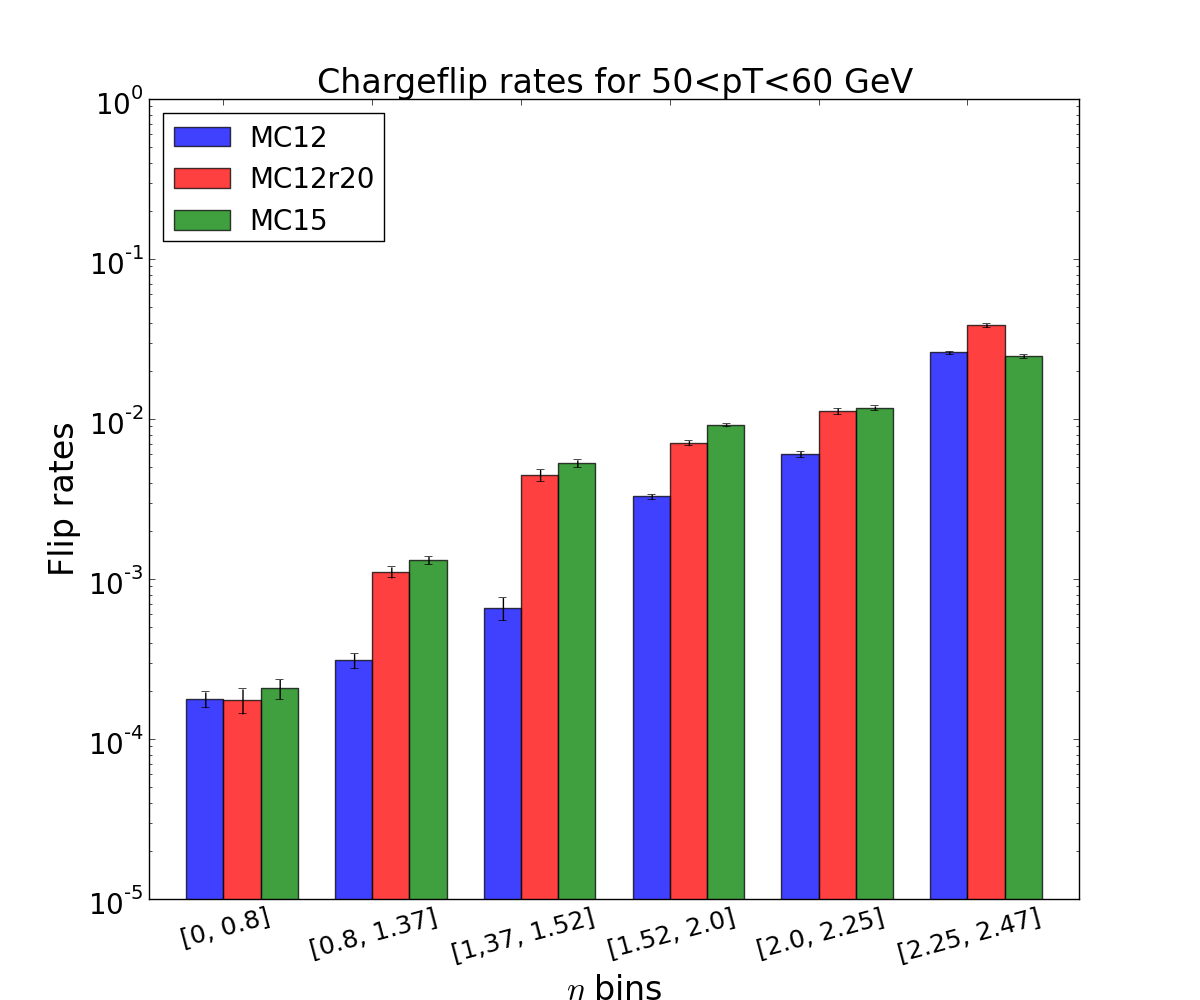
\includegraphics[width=0.33\linewidth]{FIGURES/BKG/chargeFlip/APPENDIX/fliprates_MC12r20/fliprates_3samples_50.png}
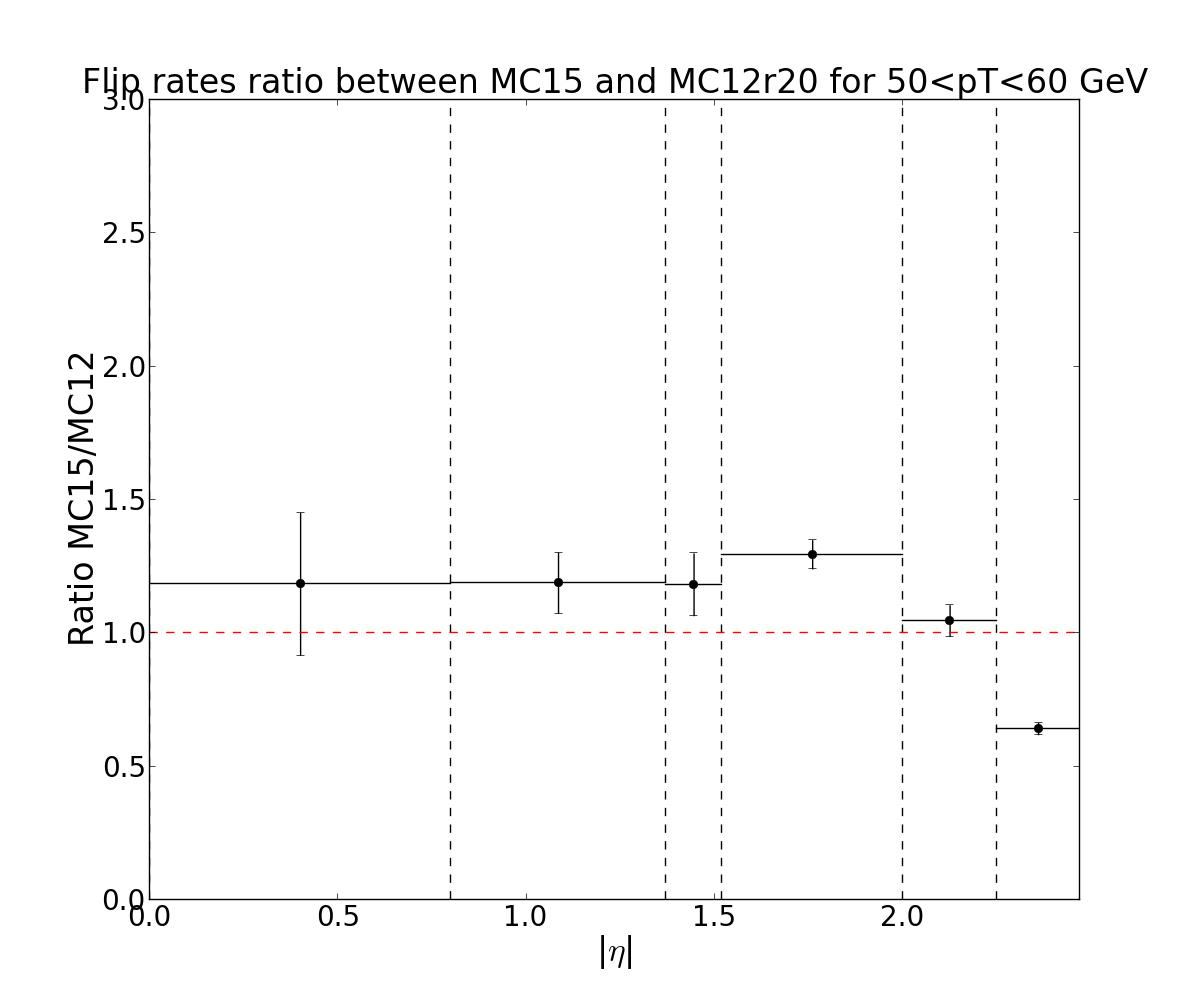
\includegraphics[width=0.33\linewidth]{FIGURES/BKG/chargeFlip/APPENDIX/ratio_MC15vsMC12r20/ratio_plot_50.png}
\vfill
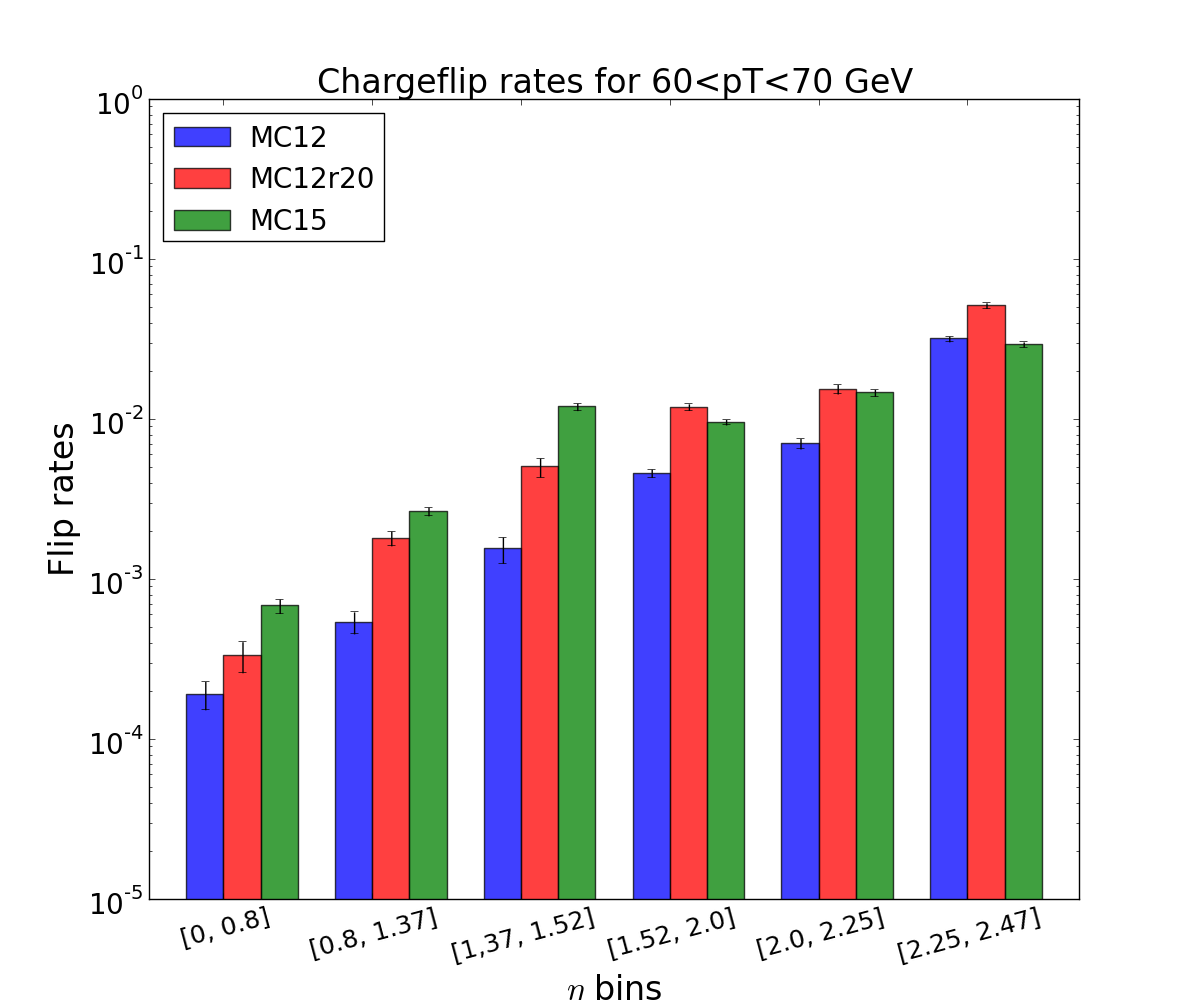
\includegraphics[width=0.33\linewidth]{FIGURES/BKG/chargeFlip/APPENDIX/fliprates_MC12r20/fliprates_3samples_60.png}
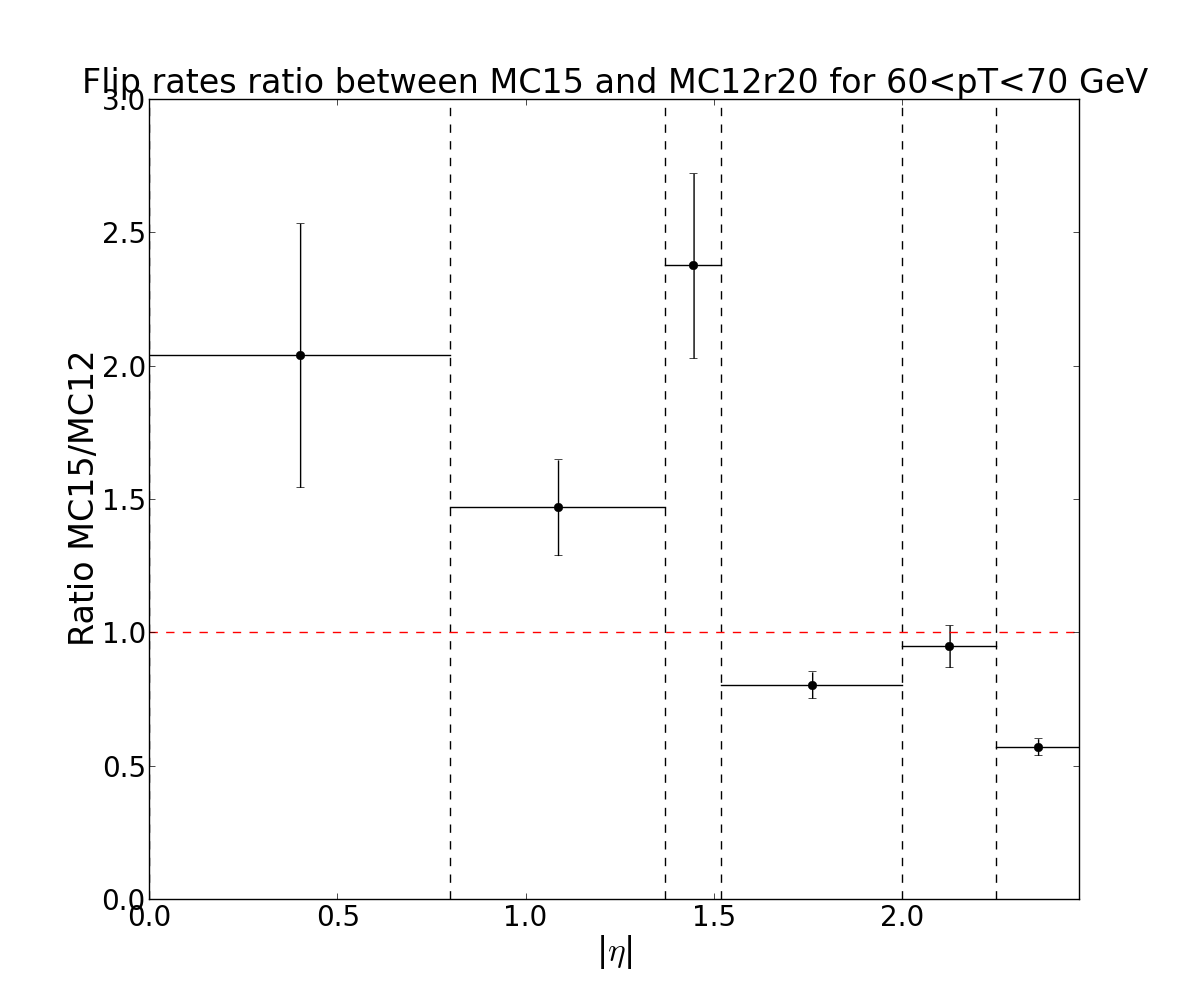
\includegraphics[width=0.33\linewidth]{FIGURES/BKG/chargeFlip/APPENDIX/ratio_MC15vsMC12r20/ratio_plot_60.png}
\caption{\label{fig:12r20vs15_2030} On the left, charge flip rates extracted from MC12 sample in blue, MC12r20 sample in red and MC15 in green. On the right, ratios between MC15 and MC12r20 charge flip rates. Only statistical uncertainties are shown.
The rates and ratios are computed for 6 different $\eta$ bins and one $\pt$ bin (from top-to bottom): $20<\pt<30$ GeV, $40<\pt<50$ GeV, $50<\pt<60$ GeV, $60<\pt<70$ GeV.}
\end{figure}

\begin{figure}[!htbp]
\centering
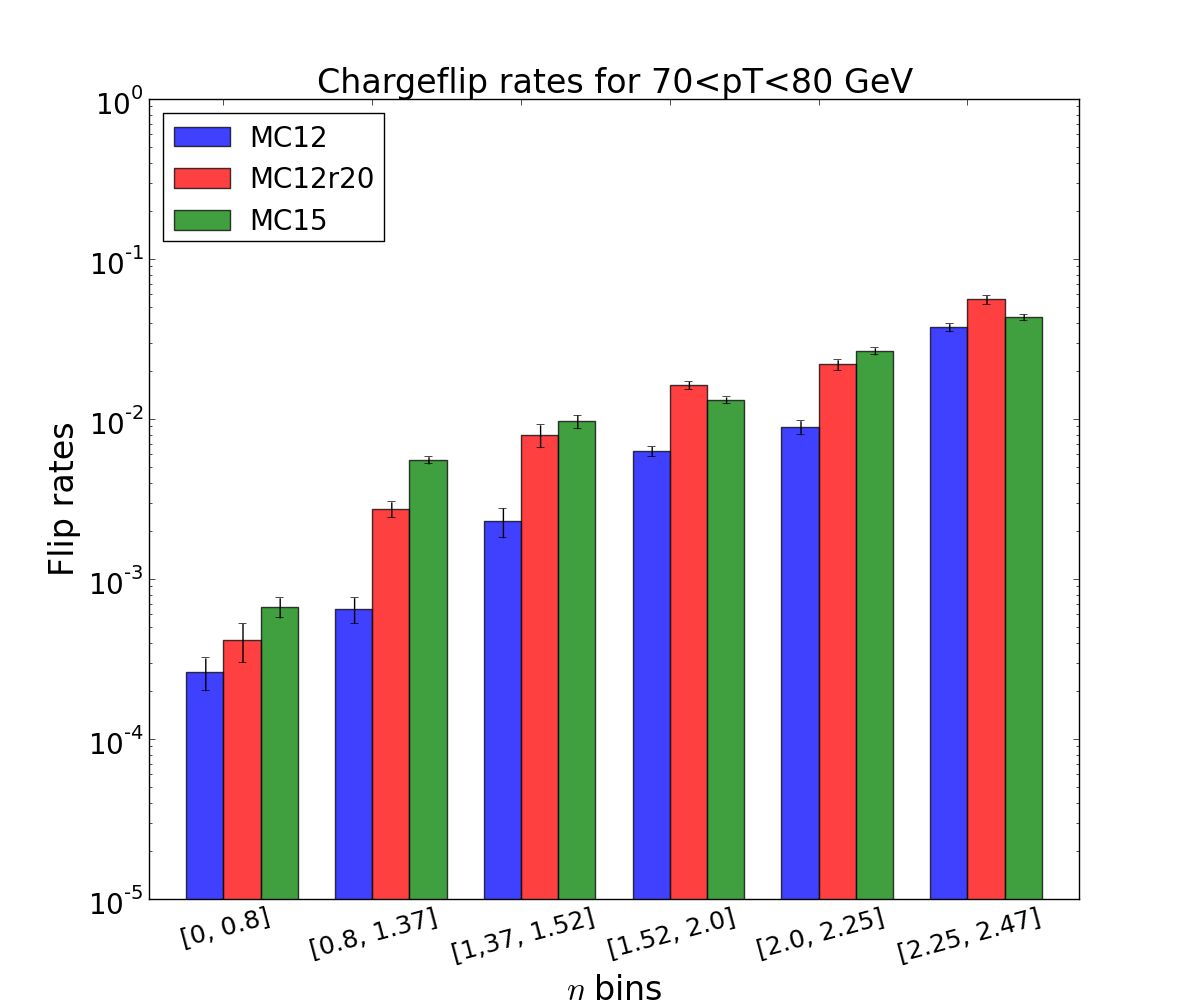
\includegraphics[width=0.33\linewidth]{FIGURES/BKG/chargeFlip/APPENDIX/fliprates_MC12r20/fliprates_3samples_70.png}
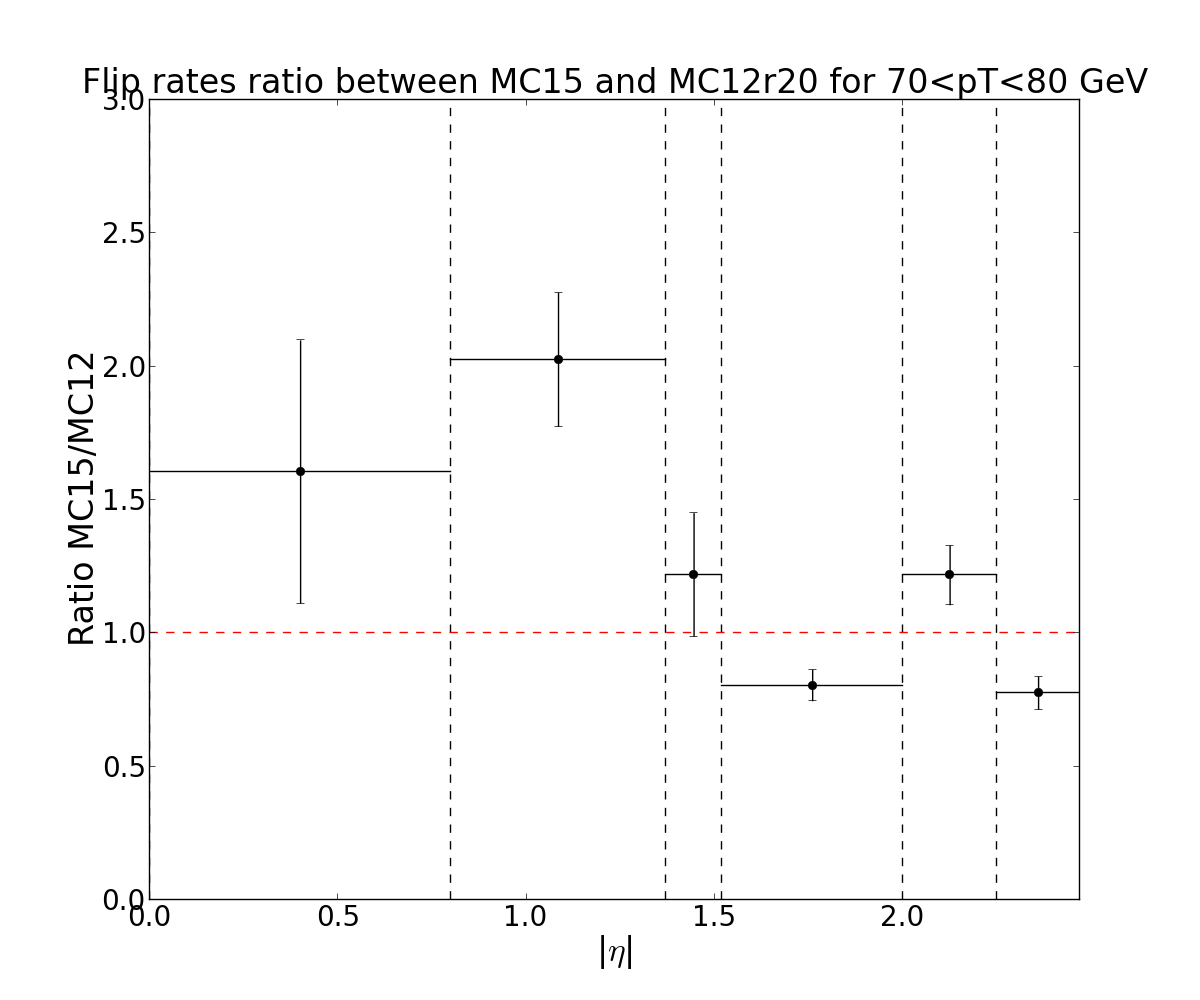
\includegraphics[width=0.33\linewidth]{FIGURES/BKG/chargeFlip/APPENDIX/ratio_MC15vsMC12r20/ratio_plot_70.png}
\vfill
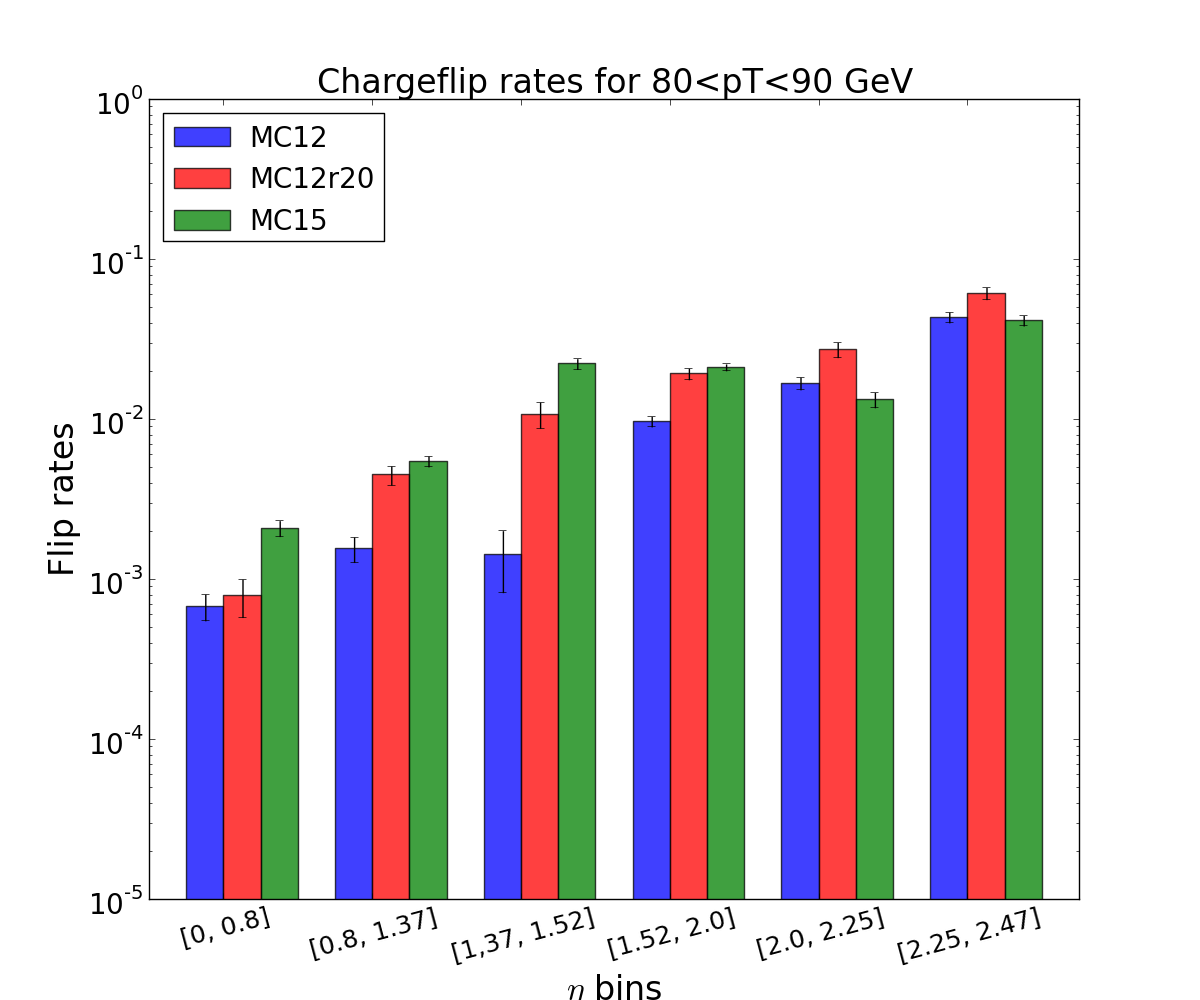
\includegraphics[width=0.33\linewidth]{FIGURES/BKG/chargeFlip/APPENDIX/fliprates_MC12r20/fliprates_3samples_80.png}
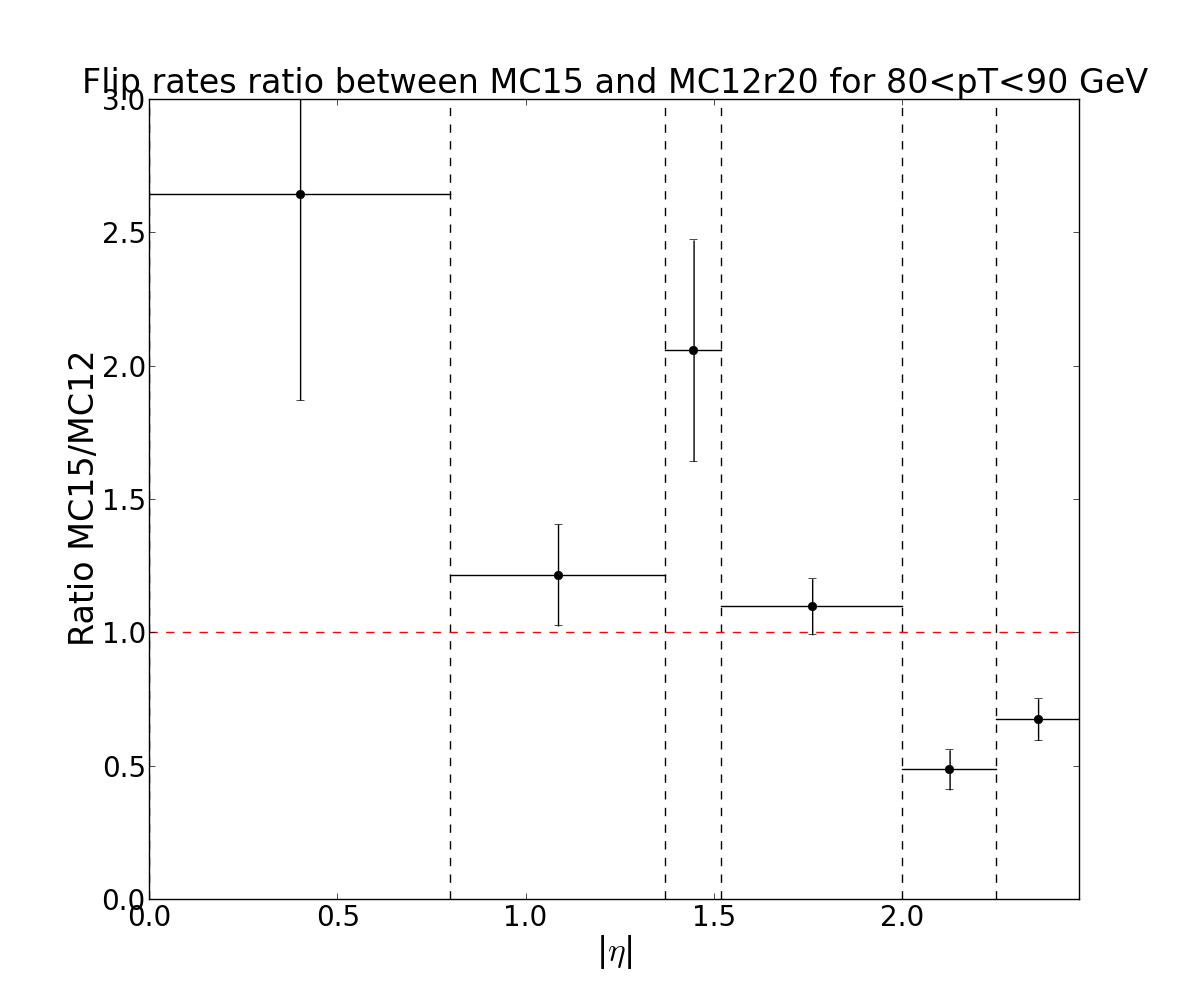
\includegraphics[width=0.33\linewidth]{FIGURES/BKG/chargeFlip/APPENDIX/ratio_MC15vsMC12r20/ratio_plot_80.png}
\vfill
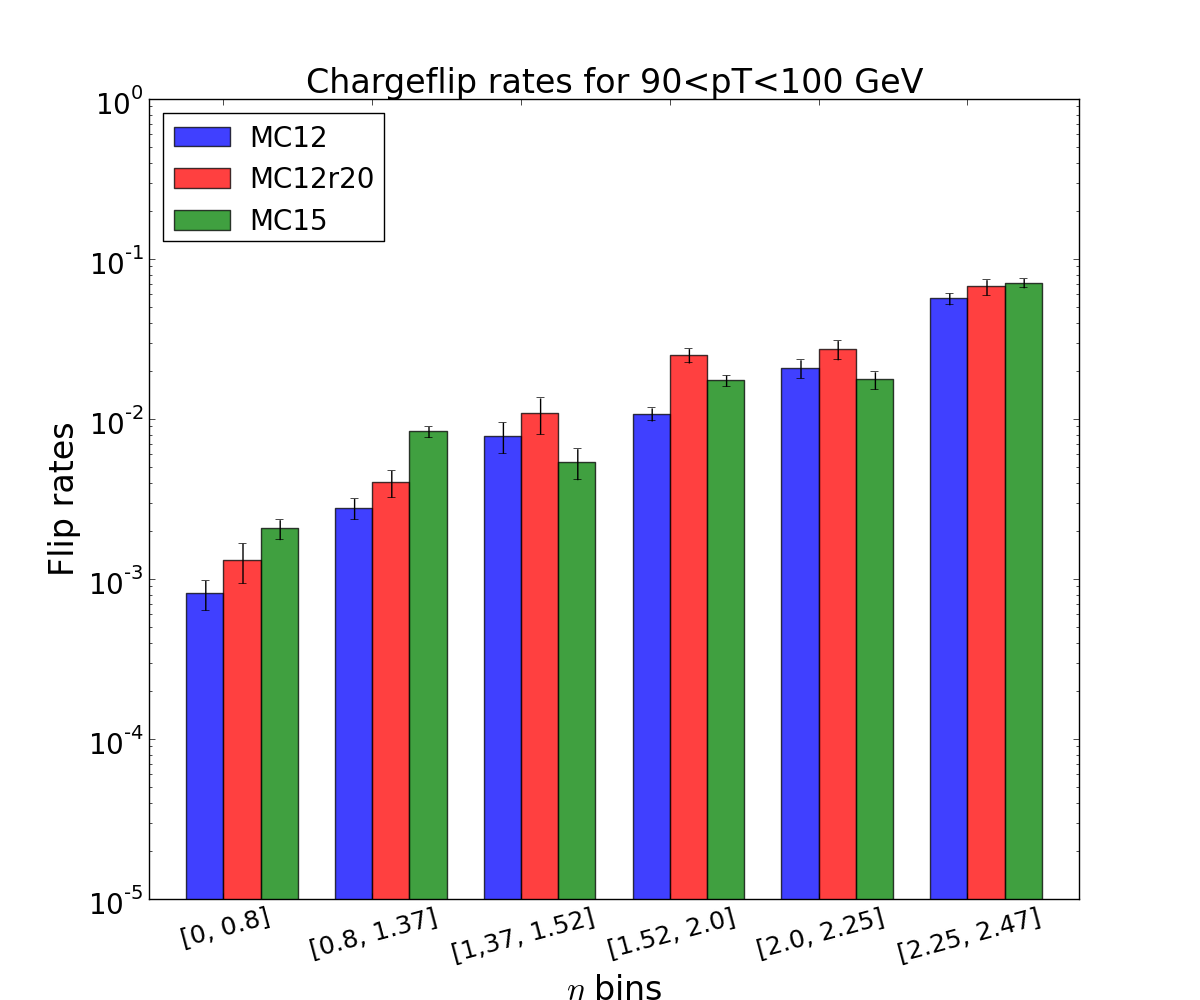
\includegraphics[width=0.33\linewidth]{FIGURES/BKG/chargeFlip/APPENDIX/fliprates_MC12r20/fliprates_3samples_90.png}
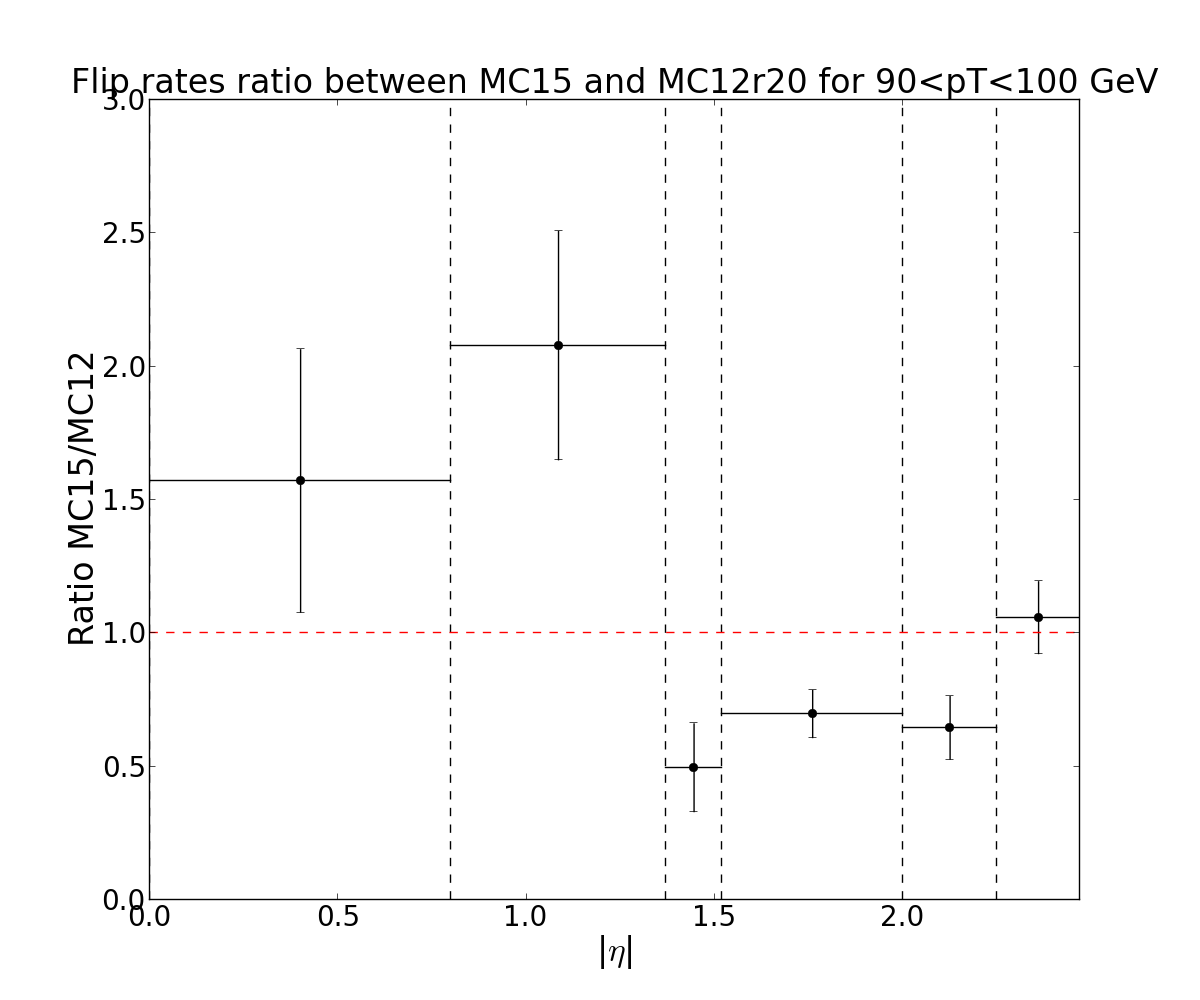
\includegraphics[width=0.33\linewidth]{FIGURES/BKG/chargeFlip/APPENDIX/ratio_MC15vsMC12r20/ratio_plot_90.png}
\vfill
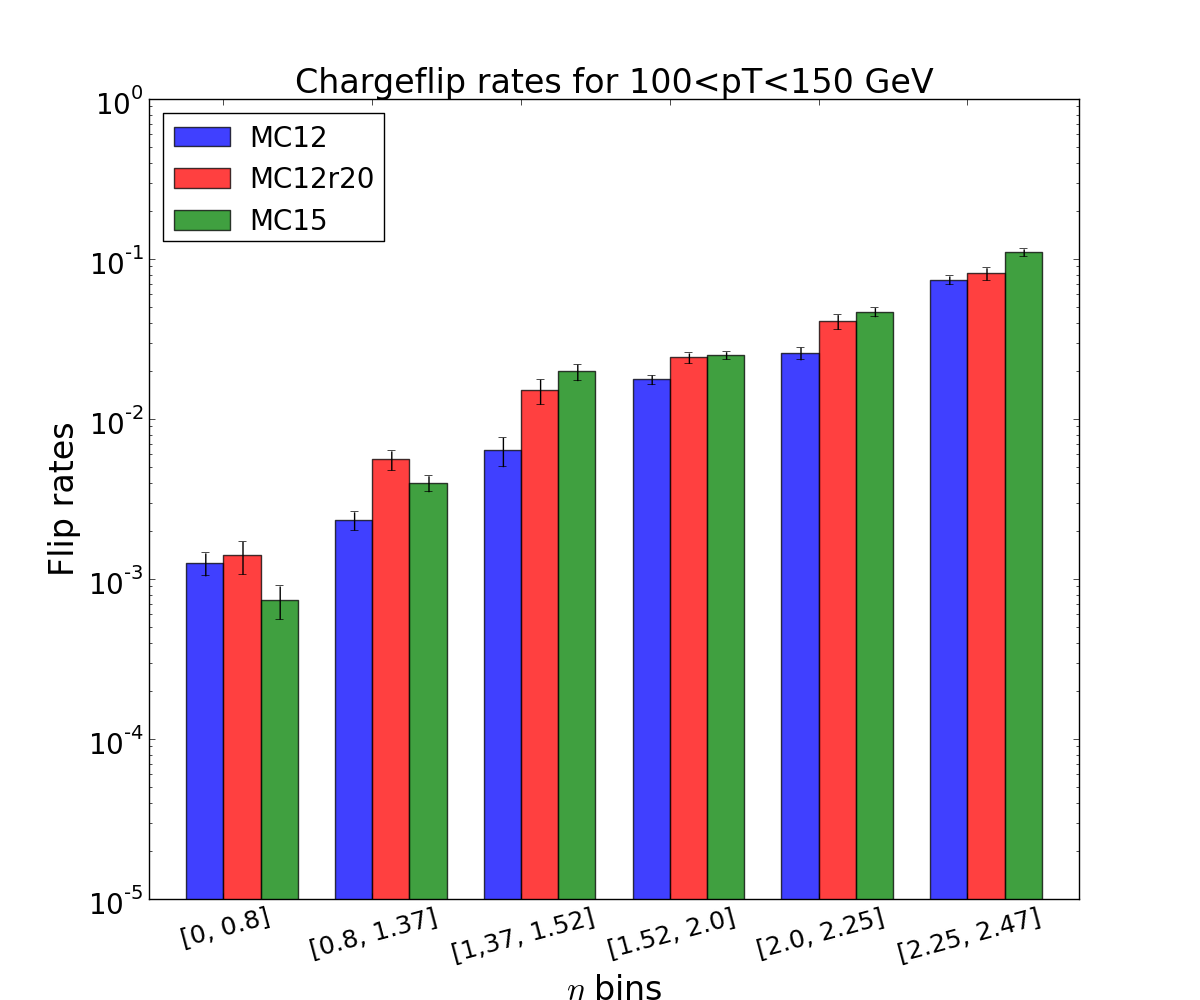
\includegraphics[width=0.33\linewidth]{FIGURES/BKG/chargeFlip/APPENDIX/fliprates_MC12r20/fliprates_3samples_100.png}
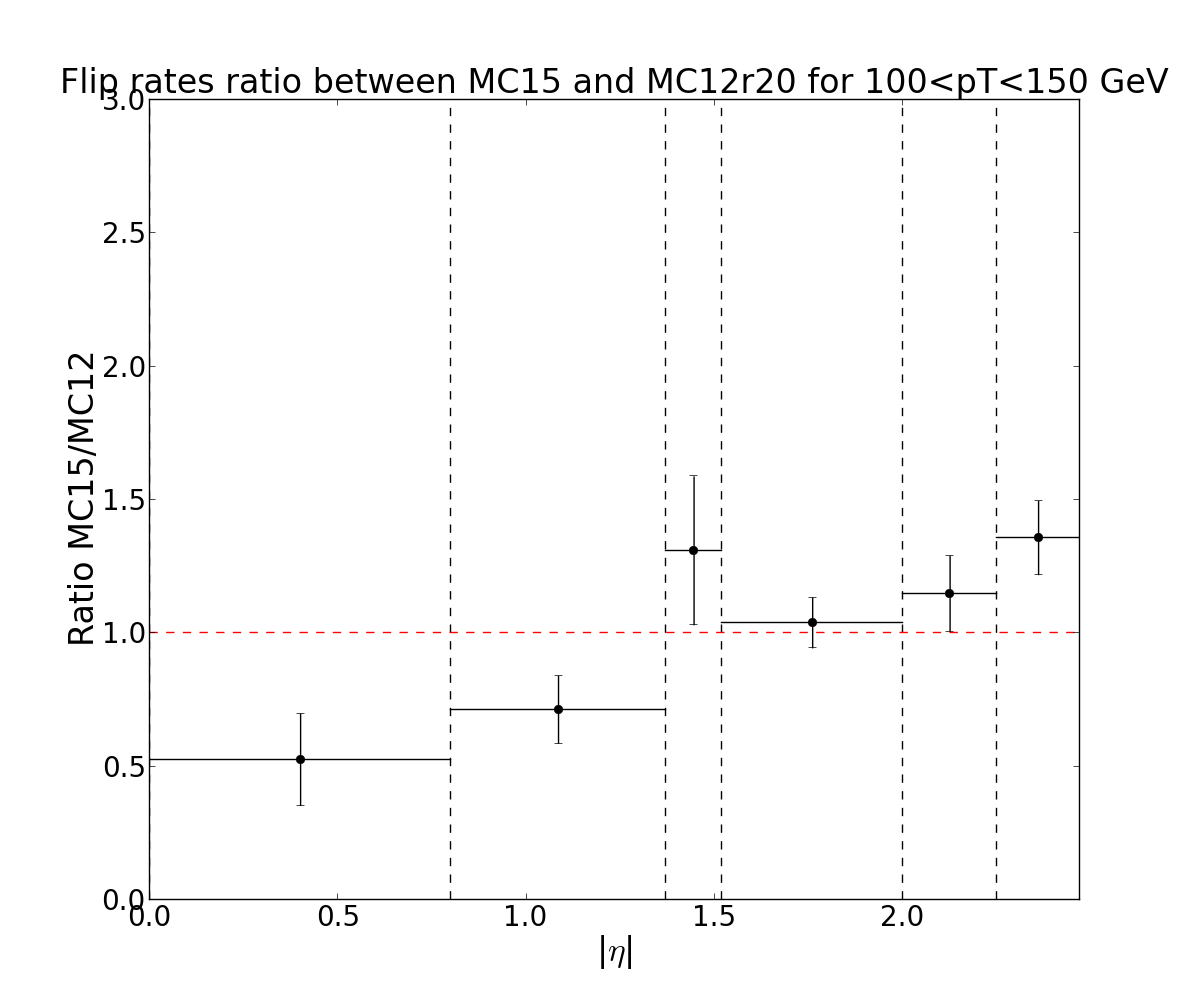
\includegraphics[width=0.33\linewidth]{FIGURES/BKG/chargeFlip/APPENDIX/ratio_MC15vsMC12r20/ratio_plot_100.png}
\caption{\label{fig:12r20vs15_7080} On the left, charge flip rates extracted from MC12 sample in blue, MC12r20 sample in red and MC15 in green. On the right, ratios between MC15 and MC12r20 charge flip rates. Only statistical uncertainties are shown. 
The rates and ratios are computed for 6 different $\eta$ bins and one $\pt$ bin (from top-to bottom): $70<\pt<80$ GeV, $80<\pt<90$ GeV, $90<\pt<100$ GeV, $100<\pt<150$ GeV.}
\end{figure}


\FloatBarrier

\subsection{Charge flip rates plots using variables $z_0$, $ptvarcone20/pT$ or $topoETcone20/pT$ as signal selection cuts}
\label{app:CFrates3}

\begin{figure}[!htbp]
\centering
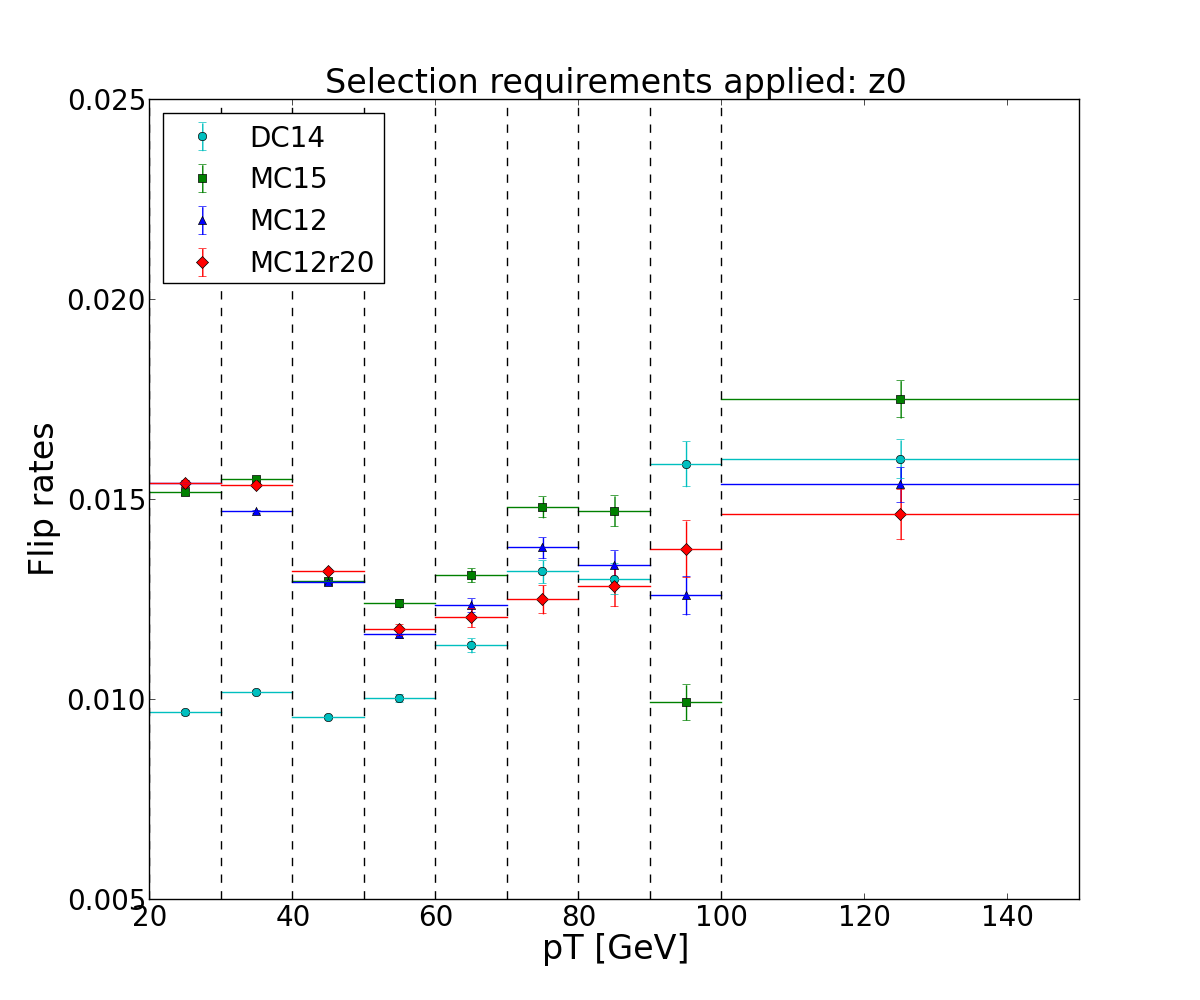
\includegraphics[width=0.4\linewidth]{FIGURES/BKG/chargeFlip/APPENDIX/fliprates_pT_z0.png}
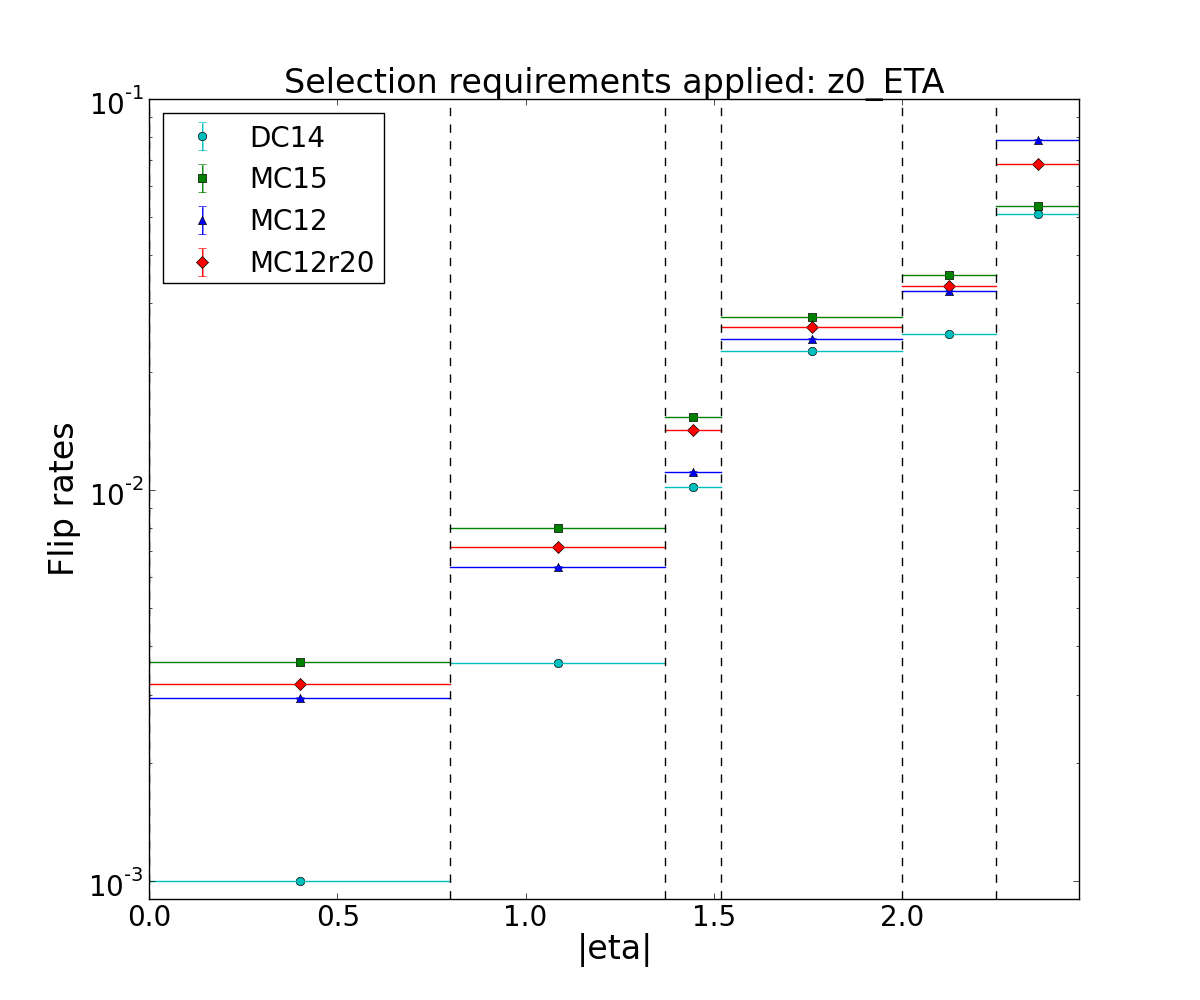
\includegraphics[width=0.4\linewidth]{FIGURES/BKG/chargeFlip/APPENDIX/fliprates_eta_z0_ETA.png}
\vfill
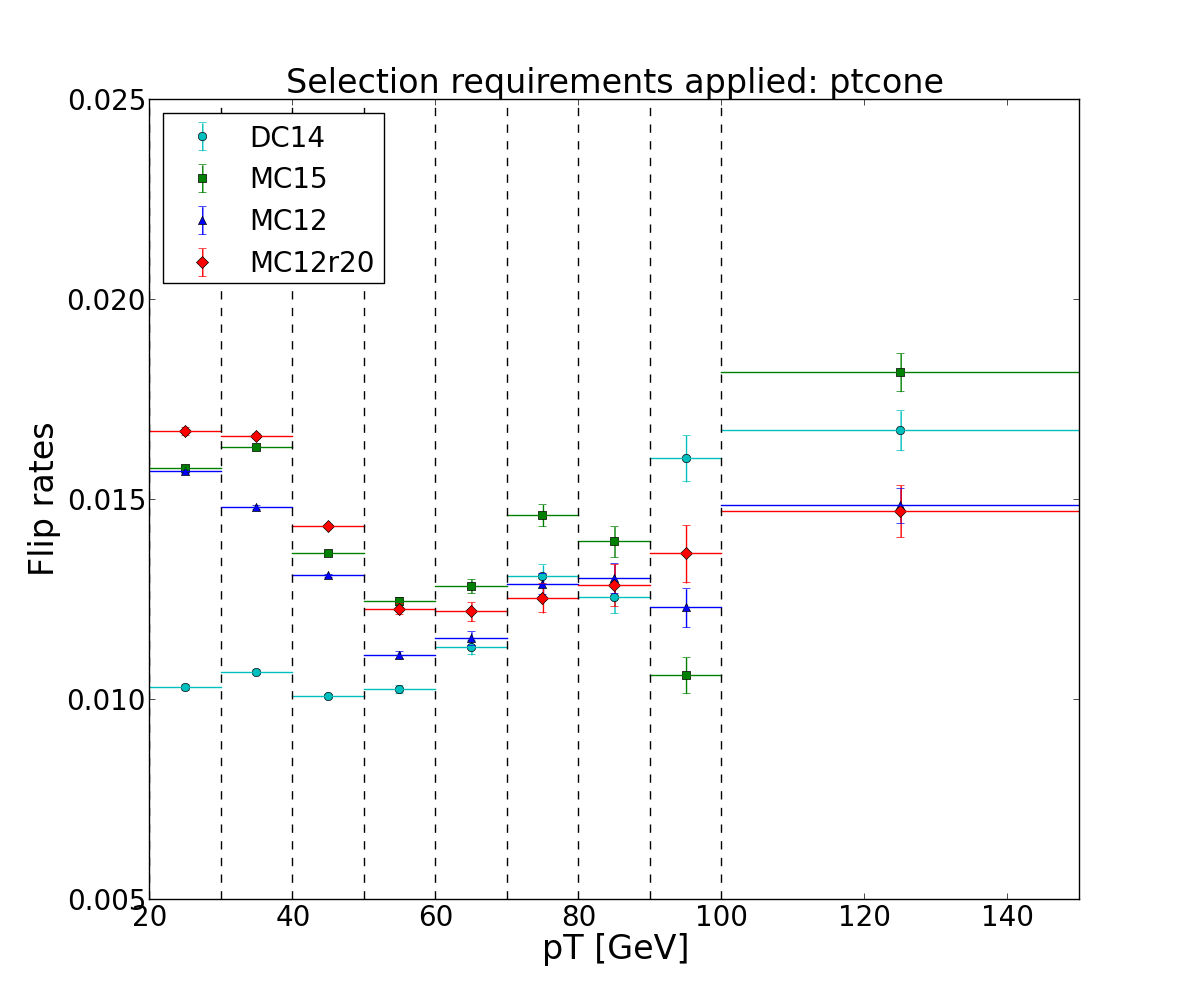
\includegraphics[width=0.4\linewidth]{FIGURES/BKG/chargeFlip/APPENDIX/fliprates_pT_ptcone.png}
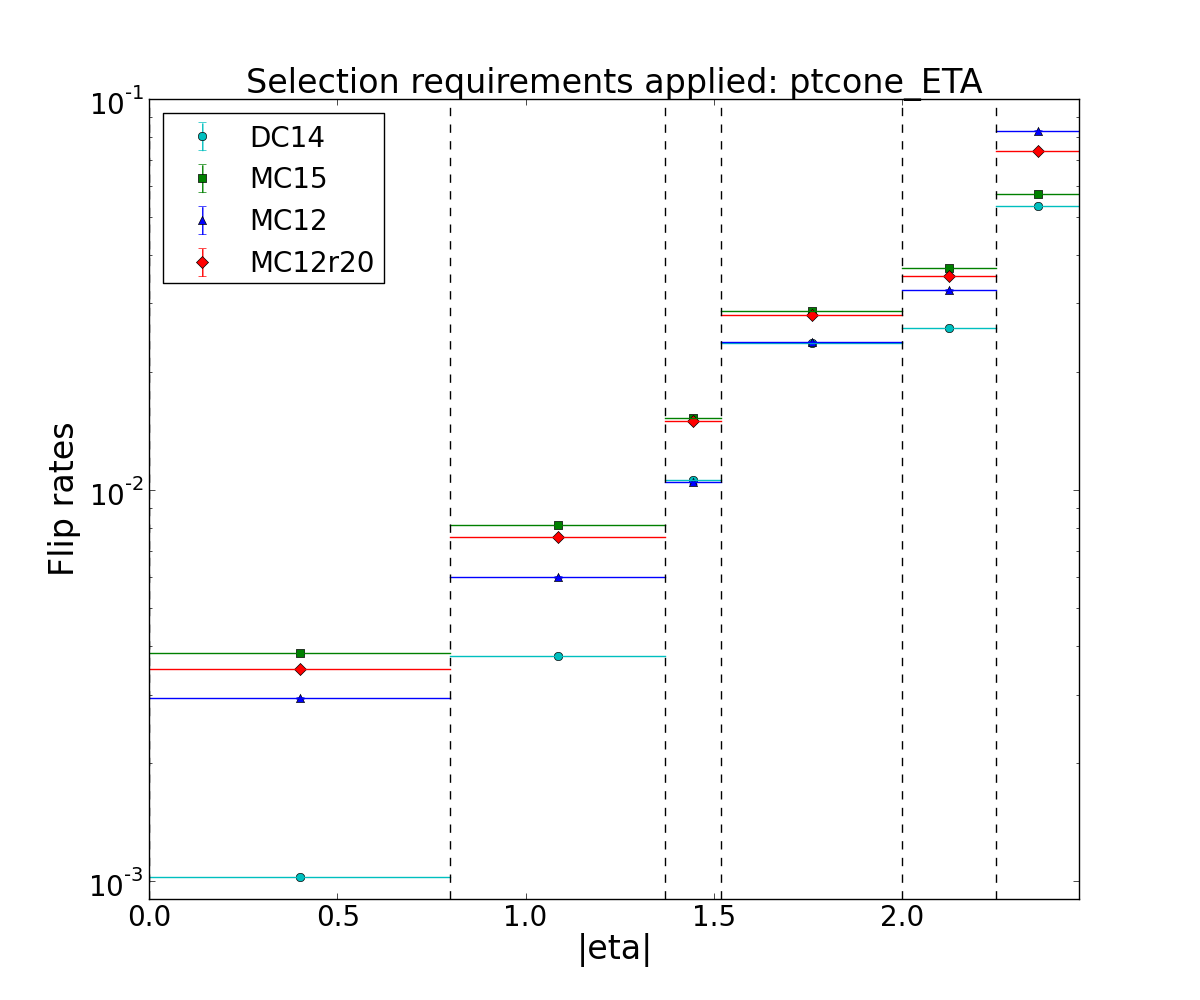
\includegraphics[width=0.4\linewidth]{FIGURES/BKG/chargeFlip/APPENDIX/fliprates_eta_ptcone_ETA.png}
\vfill
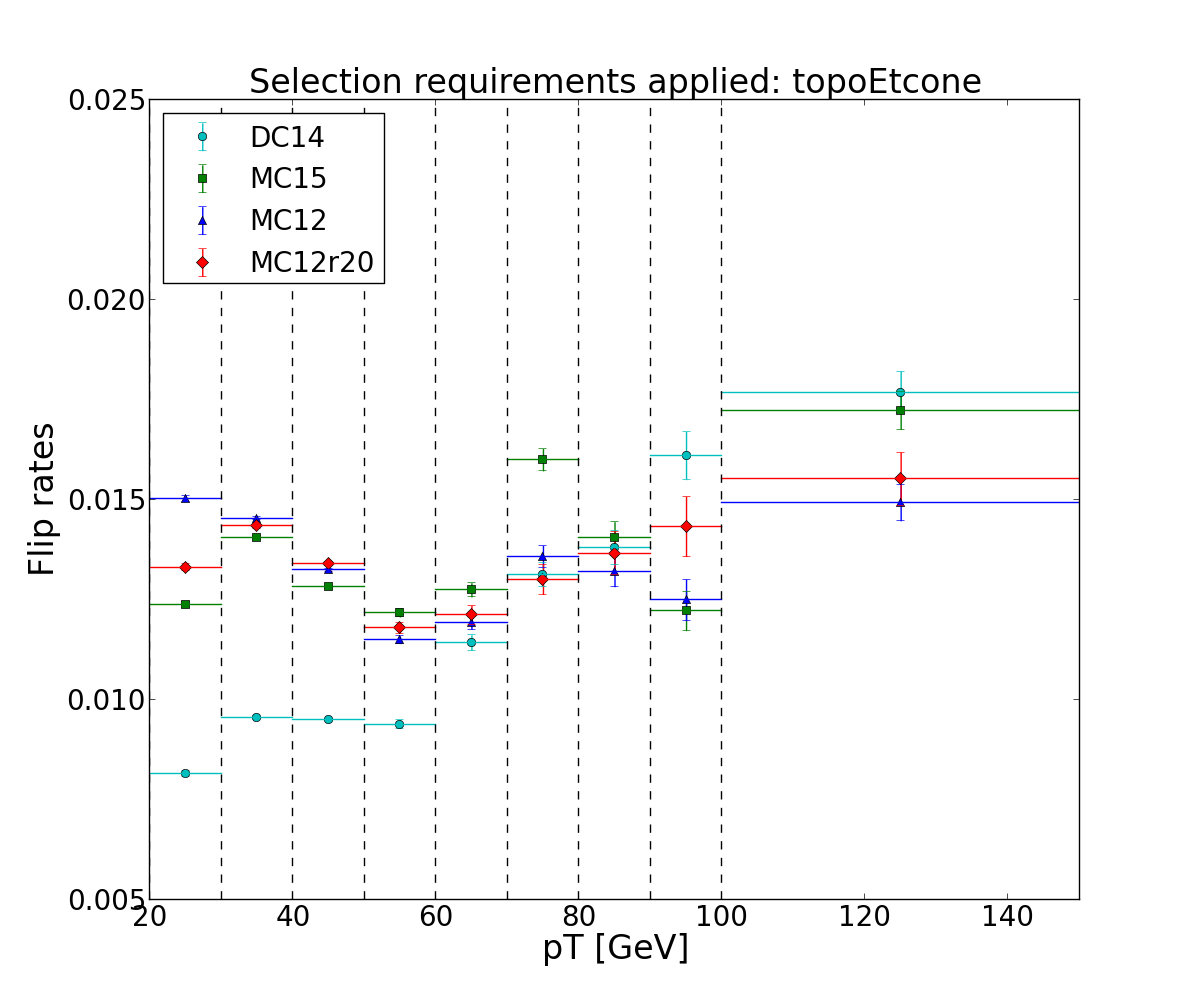
\includegraphics[width=0.4\linewidth]{FIGURES/BKG/chargeFlip/APPENDIX/fliprates_pT_topoEtcone.png}
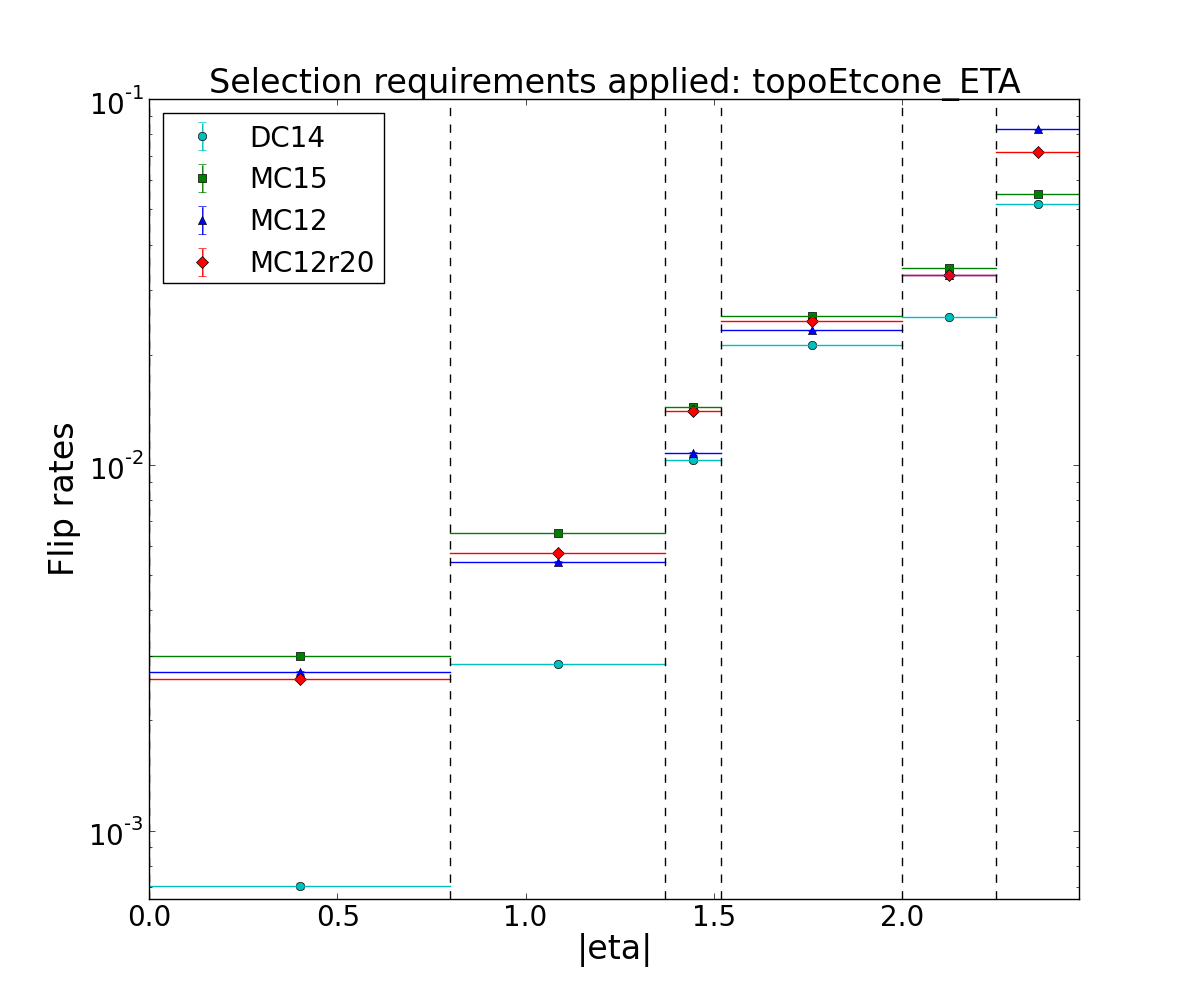
\includegraphics[width=0.4\linewidth]{FIGURES/BKG/chargeFlip/APPENDIX/fliprates_eta_topoEtcone_ETA.png}
\caption{\label{fig:ptcone} Charge flip rates extracted from different MC samples with a $\pt$ binning (left) and $\eta$ binning (right). Only statistical uncertainties are shown. On the top plots, only longitudinal impact parameter ($\left | z_0 \cdot \sin{\theta} \right |<0.4 mm $) and transverse momentum ($\pt>20$ GeV) cuts considered as signal selection cuts. On the middle ones, only track isolation ($ptvarcone20/\pt<0.06$) and transverse momentum ($\pt>20$ GeV) cuts considered as signal selection cuts and on the bottom plots only calorimeter isolation ($topoETcone20/\pt<0.06$) and transverse momentum ($\pt>20$ GeV) cuts considered as signal selection cuts.}
\end{figure}
